\documentclass[aoas, preprint]{imsart}\usepackage[]{graphicx}\usepackage[]{color}
%% maxwidth is the original width if it is less than linewidth
%% otherwise use linewidth (to make sure the graphics do not exceed the margin)
\makeatletter
\def\maxwidth{ %
  \ifdim\Gin@nat@width>\linewidth
    \linewidth
  \else
    \Gin@nat@width
  \fi
}
\makeatother

\definecolor{fgcolor}{rgb}{0.345, 0.345, 0.345}
\newcommand{\hlnum}[1]{\textcolor[rgb]{0.686,0.059,0.569}{#1}}%
\newcommand{\hlstr}[1]{\textcolor[rgb]{0.192,0.494,0.8}{#1}}%
\newcommand{\hlcom}[1]{\textcolor[rgb]{0.678,0.584,0.686}{\textit{#1}}}%
\newcommand{\hlopt}[1]{\textcolor[rgb]{0,0,0}{#1}}%
\newcommand{\hlstd}[1]{\textcolor[rgb]{0.345,0.345,0.345}{#1}}%
\newcommand{\hlkwa}[1]{\textcolor[rgb]{0.161,0.373,0.58}{\textbf{#1}}}%
\newcommand{\hlkwb}[1]{\textcolor[rgb]{0.69,0.353,0.396}{#1}}%
\newcommand{\hlkwc}[1]{\textcolor[rgb]{0.333,0.667,0.333}{#1}}%
\newcommand{\hlkwd}[1]{\textcolor[rgb]{0.737,0.353,0.396}{\textbf{#1}}}%

\usepackage{framed}
\makeatletter
\newenvironment{kframe}{%
 \def\at@end@of@kframe{}%
 \ifinner\ifhmode%
  \def\at@end@of@kframe{\end{minipage}}%
  \begin{minipage}{\columnwidth}%
 \fi\fi%
 \def\FrameCommand##1{\hskip\@totalleftmargin \hskip-\fboxsep
 \colorbox{shadecolor}{##1}\hskip-\fboxsep
     % There is no \\@totalrightmargin, so:
     \hskip-\linewidth \hskip-\@totalleftmargin \hskip\columnwidth}%
 \MakeFramed {\advance\hsize-\width
   \@totalleftmargin\z@ \linewidth\hsize
   \@setminipage}}%
 {\par\unskip\endMakeFramed%
 \at@end@of@kframe}
\makeatother

\definecolor{shadecolor}{rgb}{.97, .97, .97}
\definecolor{messagecolor}{rgb}{0, 0, 0}
\definecolor{warningcolor}{rgb}{1, 0, 1}
\definecolor{errorcolor}{rgb}{1, 0, 0}
\newenvironment{knitrout}{}{} % an empty environment to be redefined in TeX

\usepackage{alltt}

\usepackage{amsthm,amsmath,natbib}
\RequirePackage[colorlinks,citecolor=blue,urlcolor=blue]{hyperref}

% provide arXiv number if available:
\arxiv{arXiv:0000.0000}

% put your definitions there:
\startlocaldefs
\usepackage{enumitem}
\usepackage[hang, small,labelfont=bf,up,textfont=it,up]{caption} % Custom captions under/above floats in tables or figures
\usepackage{subcaption}
\usepackage{lineno}
\modulolinenumbers[5]

\usepackage{xr}
\externaldocument{imaging-supplement}

\renewcommand{\topfraction}{0.99}	% max fraction of floats at top
\renewcommand{\bottomfraction}{0.99}	% max fraction of floats at bottom
% parameters for text pages
\setcounter{topnumber}{2}
\setcounter{bottomnumber}{2}
\setcounter{totalnumber}{4}     % 2 may work better
\setcounter{dbltopnumber}{2}    % for 2-column pages
\renewcommand{\dbltopfraction}{0.9}	% fit big float above 2-col. text
\renewcommand{\textfraction}{0.07}	% allow minimal text w. figs
%   Parameters for FLOAT pages (not text pages):
\renewcommand{\floatpagefraction}{0.98}	% require fuller float pages
% N.B.: floatpagefraction MUST be less than topfraction !!
\renewcommand{\dblfloatpagefraction}{0.98}	% require fuller float pages


\newcommand{\hh}[1]{{\color{magenta} #1}}
\newcommand{\eh}[1]{{\color{blue} #1}}
\newcommand{\ac}[1]{{\color{darkgreen} #1}}

\endlocaldefs
\IfFileExists{upquote.sty}{\usepackage{upquote}}{}
\begin{document}

\begin{frontmatter}

% "Title of the paper"
\title{Automatic Matching of Bullet Lands}\thanksref{T1}
\thankstext{T1}{Resources for this manuscript, including R code to reproduce all of the models, tables and figures, can be found at  \url{https://github.com/erichare/imaging-paper}.}
\runtitle{Automatic Matching of Bullet Lands}
\runauthor{E. Hare et al.}

% indicate corresponding author with \corref{}
\begin{aug}
\author{\fnms{Eric} \snm{Hare}\corref{}\ead[label=e1]{erichare@iastate.edu}\thanksref{t1, m1}},
\author{\fnms{Heike} \snm{Hofmann}\ead[label=e2]{hofmann@iastate.edu}\thanksref{m1}}
\and
\author{\fnms{Alicia} \snm{Carriquiry}\ead[label=e3]{alicia@iastate.edu}\thanksref{m1}}

\thankstext{t1}{This research was partially funded by the Center for Statistics and Applications in Forensic Evidence (CSAFE) through Cooperative Agreement \#70NANB15H176 between NIST and Iowa State University, which includes activities carried out at Carnegie Mellon University, University of California Irvine, and University of Virginia.} 
\affiliation{Iowa State University\thanksmark{m1}}

\address{Address of the Authors\\
Department of Statistics and Statistical Laboratory\\ Snedecor Hall\\
Ames Iowa 50011-1210\\
\printead{e1}\\
\phantom{E-mail:\ }\printead*{e2}\\
\phantom{E-mail:\ }\printead*{e3}}
\end{aug}
%
\begin{abstract}
In 2009, the National Academy of Sciences published a report questioning the scientific validity of many forensic methods including firearm examination. Firearm examination is a forensic tool used to determine whether two bullets were fired from the same gun barrel. During the firing process, rifling, manufacturing defects, and impurities in the barrel create striation marks on the bullet. Identifying these striation markings in an attempt to match two bullets is the primary goal. We propose an automated framework for the analysis of the 3D surface measurements, that first transcribes the markings into a 2D plotting framework. This makes identification of matches easier and allows for a quantification of both matches and matchability of barrels. The automatic matching routine we propose manages to (a) correctly identify lands with too much damage to be suitable for matching, and (b) correctly identify all 10,384 land-to-land matches of the James Hamby study \citep{hamby:2009}.
\end{abstract}

%\begin{keyword}[class=MSC]
%\kwd[Primary ]{}
%\kwd{}
%\kwd[; secondary ]{}
%\end{keyword}

\begin{keyword}
\kwd{3D Topological Surface Measurement}
\kwd{Data visualization}
\kwd{Machine Learning}
\kwd{Feature importance}
\kwd{Cross-correlation function}
\end{keyword}

\end{frontmatter}

\linenumbers
%\tableofcontents
%\newpage



\section{Introduction}
%\hh{
%Todo list for journal shape-up: there is a lot of good material, we mainly need to focus on what story to tell and make that a solid argument.
%\begin{enumerate}
%\item take out a few things: no circular fit, no figures 9 and 10 
%\item do we need the web app?
%\item out: lots of the figures can go into a supplement, together with a discussion. In the paper we then have a summary of what can be seen, so that we can focus on the results. 
%\item add: formula for loess fit and its s.e.
%\item add: comparison of error rates to those of FEs in Hamby study.
%\item change: emphasis in varying cross section. once a stable region is found, how little change is happening? 
%\item add: Why do we take the lowest stable cross section?
%\item add: more discussion of the density plots: probability ratio for a match - exchanged probability ratios for ROC curves
%\item add: more discussion on additional bullet images. NIST database claims to have 70 bullets -- that would be two sets of the study, but only 35 bullets are currently available. Should we contact Alan Zheng to see whether we can get access to more bullet files? Not enough space for this one.
%\item add: we could extend the results of the James Hamby study by trying to match every single land against all other lands. This would almost double the number of comparisons ($21,115 = (118+88)\cdot 205/2$). Something for the appendix? What would be fun, would be to show all of the aligned signatures for all ten barrels. (moved to supplement)
%\item add: should we add a paragraph on the speed of the evaluation? - separate out into pre-processing (needs to be done once) and matching (pairwise comparison of lands). If we only do bullet matching, we could speed this process up by eliminating some land comparisons. - Thinking about this more, I'm against it. The speed massively depends on the kind of computer used - the important thing is, that on a server all of these calculations are very fast -- even my machine can do 11 comparisons per second, if the files are pre-processed. Pre-processing might take a couple of seconds - at most 20-30 seconds for each bullet land. That is an initial cost one has to pay.
%\item add: we might need a proper definition of the joint striation marks (the result of striation-identify)
%\item change: we could make the table into a labelled dotplot of importance to save space. We don't need the mean and standard deviations anymore -- the density plots and the ROCs take care of that.
%\item change: the focus of the paper is initially quite strongly on the maximal consecutively matching striae (CMS). We need to emphasis the role of CMS in the introduction: max CMS is Biasotti's main criterium for matching.  max CMS is part of current practice (AFTE criteria citation). AFIS \cite{AFIS} is suggesting it for an automated system (was there ever a phase II of that project?). Problem is, that determining CMS is subjective; counting CMS in particular, has been found to be subjective to the examiner: `the concept of counting striations is subjective and based on experience'~\citep{miller:1998}.  For an automatic routine we are faced with the problem of having to determine what a stria is. XXX Should we include one of those microscopic images to bring that point home? We would need somebody qualified to tell us how many CMS there are, though.
%\item to consider: AOAS states that accepted papers rarely have more than 20 pages. We are currently over by a couple of pages.
%\item definitions: 
%A bullet's {\it signature} is defined as the residual surface measurements after removing the big structure using the loess fit. The {\it cross section} defines the location along the $x$ axis  at which the signature is taken.
%\end{enumerate}
%}
Firearm examination is a forensic tool used to determine whether two bullets were fired from the same gun barrel. This process has broad applicability in terms of  convictions  in the United States criminal justice system. Ballistics identification has long been considered an accepted and reliable procedure, but in the past ten years has undergone more significant scrutiny. In 2005, in \emph{United States vs. Green}, the court ruled that the forensic expert could not confirm that the bullet casings came from a specific weapon with certainty, but could merely ``describe" other casings which are similar. Further court cases in the late 2000s expressed caution about the use of ballistics identification evidence~\citep{giannelli:2011}.

In 2009, the National Academy of Sciences published a report~\citep{NAS:2009} questioning the scientific validity of many forensic methods including firearm examination. The report states that ``[m]uch forensic evidence -- including, for example, bite marks and firearm and toolmark identification is introduced in criminal trials without any meaningful scientific validation, determination of error rates, or reliability testing to explain the limits of the discipline."

Rifling, manufacturing defects, and impurities in a barrel create striation marks on the bullet during the firing process. These marks are assumed to be unique to the barrel, as described in a 1992 AFTE article~\citep{afte:1992}. ``The theory of identification as it pertains to the comparison of toolmarks enables opinions of common origin to be made when the \emph{unique surface contours} of two toolmarks are in sufficient agreement" The article goes on to state that ``Significance is determined by the comparative examination of two or more sets of surface contour patterns comprised of individual peaks, ridges and furrows."

From a statistical standpoint, identification of the gun that fired the bullet(s) requires that we compare the probabilities of observing matching striae under the competing hypotheses that the gun fired, or did not fire, the crime scene bullet. If indeed the uniqueness assumption is plausible, the latter probability approaches zero.

Current standard practice~\cite{afte:1992} relies in part on the assessment of the so-called maximal number of consecutively matching striae (CMS), first defined by \citet{biasotti:1959}.
One of the problems is that a human inspection to determine CMS is subjective \citep{miller:1998}. 

Here, we focus on the question of defining what constitutes a match, since there is no agreement in the forensics community. We propose a framework which allows for the automatic analysis of the surface topologies of bullets, and the transcription of the individual characteristics into a 2D plotting framework. 
This allows for an objective and quantitative assessment of striae-based bullet matches.

%\hh{XXX More detailed discussion of automatic approaches and database discussion XXX}

Throughout this paper, we work with images from the James Hamby Consecutively Rifled Ruger Barrel Study~\citep{hamby:2009}. Ten consecutively rifled Ruger P-85 pistol barrels were obtained from the manufacturer and fired to produce 20 known test bullets and 15 unknown bullets for comparison. 
3D topographical images of each bullet were obtained using a NanoFocus lens at 20x magnification and made publicly available on the NIST Ballistics Database Project\footnote{\url{http://www.nist.gov/forensics/ballisticsdb/hamby-consecutively-rifled-barrels.cfm}} in a format called x3p (XML 3-D Surface Profile). x3p is a container format conforming to the ISO5436-2 standard\footnote{\url{http://sourceforge.net/p/open-gps/mwiki/X3p/}}, implemented to provide a simple and standard conforming way to exchange 2D and 3D profile data. x3p was adopted by the OpenFMC (Open Forensic Metrology Consortium\footnote{\url{http://www.openfmc.org/}}), a group of academic, industry, and government firearm forensics researchers whose aim is to establish best practices for researchers using metrology in the forensic sciences.

\begin{figure}[hbtp]
  \centering
\begin{subfigure}[t]{\textwidth}\centering
\caption{View of the data along the circumference of the bullet (circular segment of about 30 degrees).\label{fig:sidex3p}}{%
      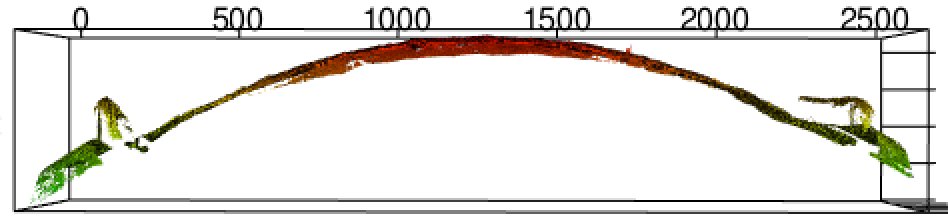
\includegraphics[width=.65\textwidth]{sidex3p.png}
      \hspace{1cm}
      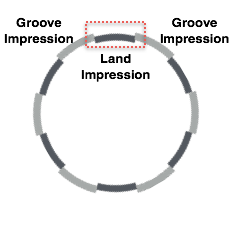
\includegraphics[width=.25\textwidth]{side-sketch.png}
    }
\end{subfigure}    
\begin{subfigure}[t]{\textwidth}\centering
    \caption{Frontal view of a bullet land (lower end of the view is the bottom of the bullet). \label{fig:topx3p}}{%
    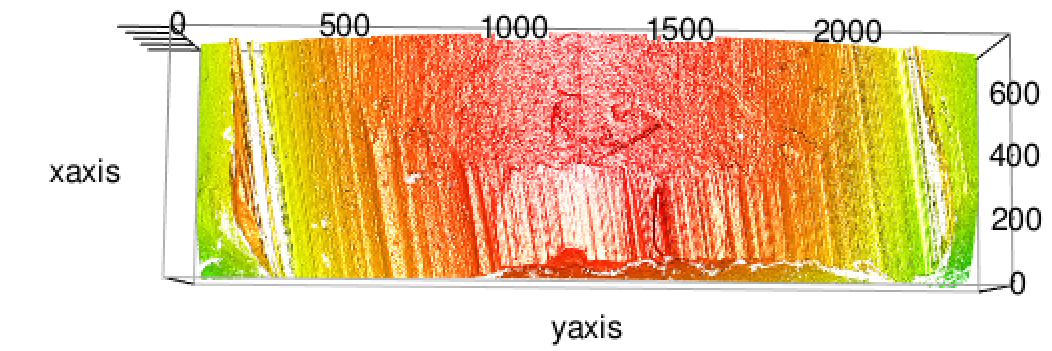
\includegraphics[width=.65\textwidth]{topx3p.png} \hspace{1cm}
    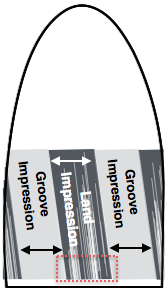
\includegraphics[width=.15\textwidth]{top-sketch.png}
    }
\end{subfigure}
\caption{Example of a groove-to-groove scan of a bullet land. The red-dotted rectangle on the right shows the location and orientation of the segment. }
\end{figure}
Each fired bullet is provided in the form of a set of six x3p files, where each file is a surface scan between adjacent grooves on the bullet, called a ``land". For notational simplicity, we refer to a particular land of some bullet as bullet X-Y, where X is the bullet identifier, and Y is the land number. An example of plotting one of these lands is given in Figures~\ref{fig:sidex3p} and~\ref{fig:topx3p}. These figures show side and top profiles of the land respectively. The tilt of the lines to the left in Figure~\ref{fig:topx3p} is not an artifact, but a direct and expected consequence of the spin induced by the rifling during the firing process. Depending on whether a barrel is rifled clockwise or counter-clockwise, the striations have a left or right tilt. The direction of the rifling is a class characteristic, i.e.\ a feature that pertains to a particular class of firearms, and is not unique at the individual barrel/bullet level.

The purpose of our paper is to present an automatic matching routine that allows for a completely objective assessment of the quality of a match. 
The original paper on the complete Hamby study already reports the successful use of several computer-assisted methods; aside from a zero false positive rate no further details on a false-negative error rate for bullets are given nor are error rates for land-to-land matches mentioned. 
% Hamby study: automated systems were successfully used for matching:
%  Intelligent Automation's SciClops - Dr. Ben Bachrach (Maryland, United States);
% Automated Land Identification System (ALIS) - Mr. Tsuneo Uchiyama (Tokyo, Japan);
% Integrated Ballistics Identification System (IBIS) – Mr. Robert Thompson (California, United States);
% BulletTRAX-3DTM - Forensic Technology Scientists (Montreal, Canada) (2 sets)
 
A procedure for bullet matching using the BulletTrax3D system is described in \citet{roberge:2006}. This study is based on another set of ten consecutively rifled barrels; matches are identified based on a bullet-to-bullet correlation score. The authors state that this process `could be automated', but no implementation of the algorithm is available. 

The remainder of this paper is structured as follows: We first discuss two methods of modeling the class structure of the bullet surfaces. %We then describe a web application for visualizing and working with bullet surfaces. 
We then proceed to describing an automatic matching routine which we evaluate on the bullets made available through the Hamby study.


\section{Bullet signatures}

In an approach to analyze the striation pattern we extract a \emph{bullet profile} \citep{ma:2004} by taking a cross section of the surface measurements at a fixed height $x$ along the bullet land.
%An initial naive approach to analyzing the striation patterns leads us to fixing a particular value of a coordinate, and then producing a plot of the surface measurements across. 
Figure \ref{fig:fixedX} shows a plot of the side profile of a bullet land. It can be seen that the global structure of the land dominates the appearance of the plot. The grooves can be clearly identified on the left and right side, and the curvature of the surface is the most visible feature in the middle.

\begin{figure}[hbtp]
  \centering
\begin{knitrout}
\definecolor{shadecolor}{rgb}{0.969, 0.969, 0.969}\color{fgcolor}
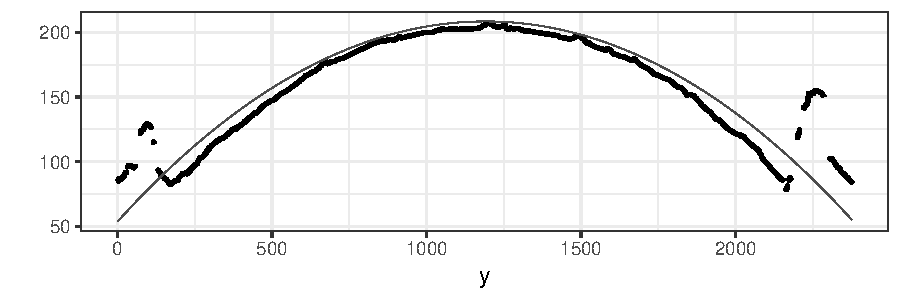
\includegraphics[width=0.65\textwidth]{fixedX-1} 

\end{knitrout}
\caption{\label{fig:fixedX}Side profile of the surface measurements (in~$\mu m$) of a bullet land at a fixed height $x$. Note that the global features dominate any deviations, corresponding to the individual characteristics of striation marks.}
\end{figure}

The smooth curve on the plot represents a segment of a perfect circle with the same radius as the bullet. While the circle is an obvious first choice for fitting the structure, it does not completely capture the bullet surface after it was fired. A discussion of a circular fit and the remaining residual structure can be found in Supplement section~\ref{supp:cylindrical}.
%It is clear that our next approach must be to model the overall structure in order to focus on the deviations, given that the deviations should correspond to bullet markings. 

%\subsection{Loess Fit}
Instead of a circular fit, we use multiple loess fits to model the overall structure and extract the bullet markings. 

\subsection{Identifying groove locations}
%In an attempt to improve upon the previous algorithm, w
We first have to identify the locations of the left and right  groove in the image. The grooves are not assumed to contain information relevant for determining matches. They also dominate the structure, and therefore need  to be removed.  
Fortunately, the location and appearance of the grooves in the surface profiles is quite consistent.
Surface measurements reach local maxima around the peak of the groove at either end of the range of $y$, we can then follow the descent of the surface measurements inwards to the valley of the groove. 
The location of the valleys  mark the points at which we should trim the image. The procedure can be described as follows:

\begin{enumerate}
    \item At a fixed height $x$ extract a bullet's profile (Figure~\ref{fig:loess_step1}, with $x = 243.75\mu m$).
    \item For each $y$ value, smooth out any deviations occurring near the minima by twice applying a rolling average with a pre-set \emph{smoothing factor} $s$. (Figure~\ref{fig:loess_step3}, smoothing factor $s = 35$ corresponding to 55$\mu m$).
%    \item For each smoothed $y$ value, compute another rolling average using the same smoothing factor as above. (Figure~\ref{fig:loess_step3}).
    \item Determine the location of the peak of the left groove by finding the first doubly-smoothed value $y_i$ that is the maximum within its smoothing window (e.g.\ such that $y_i > y_{i - 1}$ and $y_i > y_{i + 1}$, where $i$ is between 1  and $\lfloor s/2 \rfloor$). We call the location of this peak $p_{\ell}$ (see Figure~\ref{fig:loess_step47}). 
    \item Similarly, determine the location of the valley of the left groove by finding the first double-smoothed $y_j$ that is the minimum within its smoothing window. Call the location of this valley $v_{\ell}$.
    \item Reverse the order of the $y$ values and repeat the previous two steps to find the peak and valley of the right groove, $(p_{r}, v_{r})$.
    \item Trim the surface measurements to values within the two grooves (i.e.\ remove all records with $y_i < v_{\ell}$ and $y_i > v_{r}$) (see Figure~\ref{fig:loess_step47}).
\end{enumerate}

\begin{figure}[hbtp]
  \centering
\begin{subfigure}[t]{\textwidth}\centering
\caption{\label{fig:loess_step1}Step 1 of identifying groove locations: For a fixed height ($x = 243.75\mu m$)  surface measurements for bullet~1-5 are plotted across the range of $y$.}
\begin{knitrout}
\definecolor{shadecolor}{rgb}{0.969, 0.969, 0.969}\color{fgcolor}
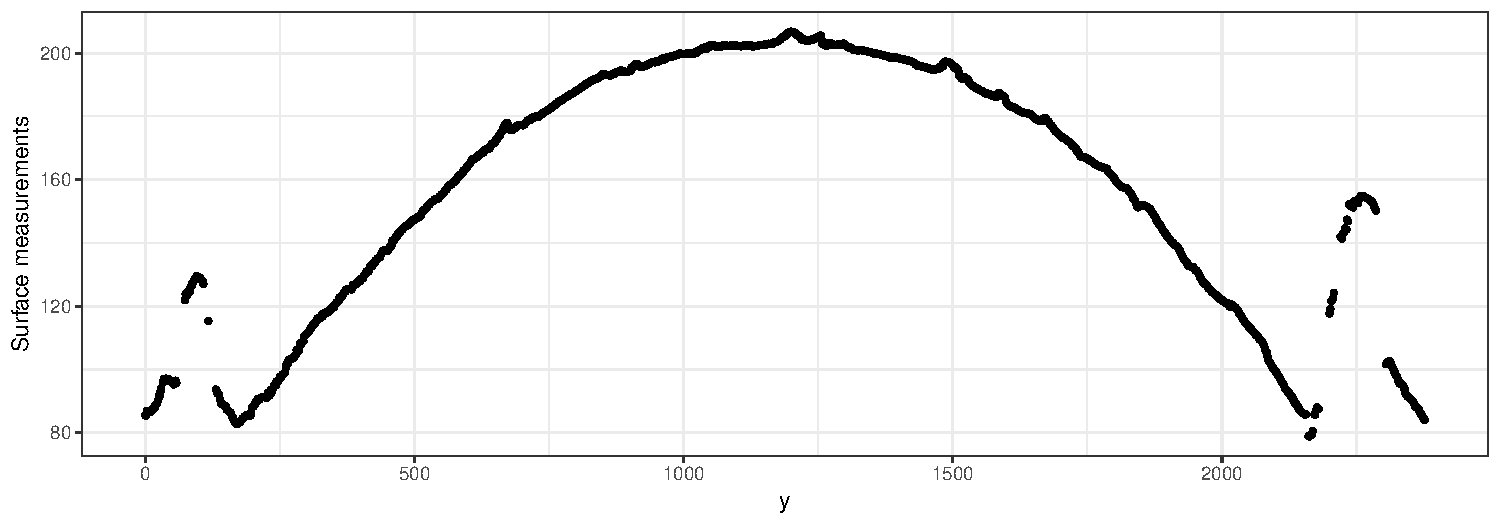
\includegraphics[width=.5\textwidth]{loess_step1-1} 

\end{knitrout}
\end{subfigure}
\begin{subfigure}[t]{\textwidth}\centering
\caption{\label{fig:loess_step3}Step 2 of identifying groove locations: The  surface measurements are smoothed twice with a smoothing factor of $s = 35$. The orange rectangle shows an example of the smoothing window. Valleys and peaks are detected, if they are not within the same window.}
\begin{knitrout}
\definecolor{shadecolor}{rgb}{0.969, 0.969, 0.969}\color{fgcolor}
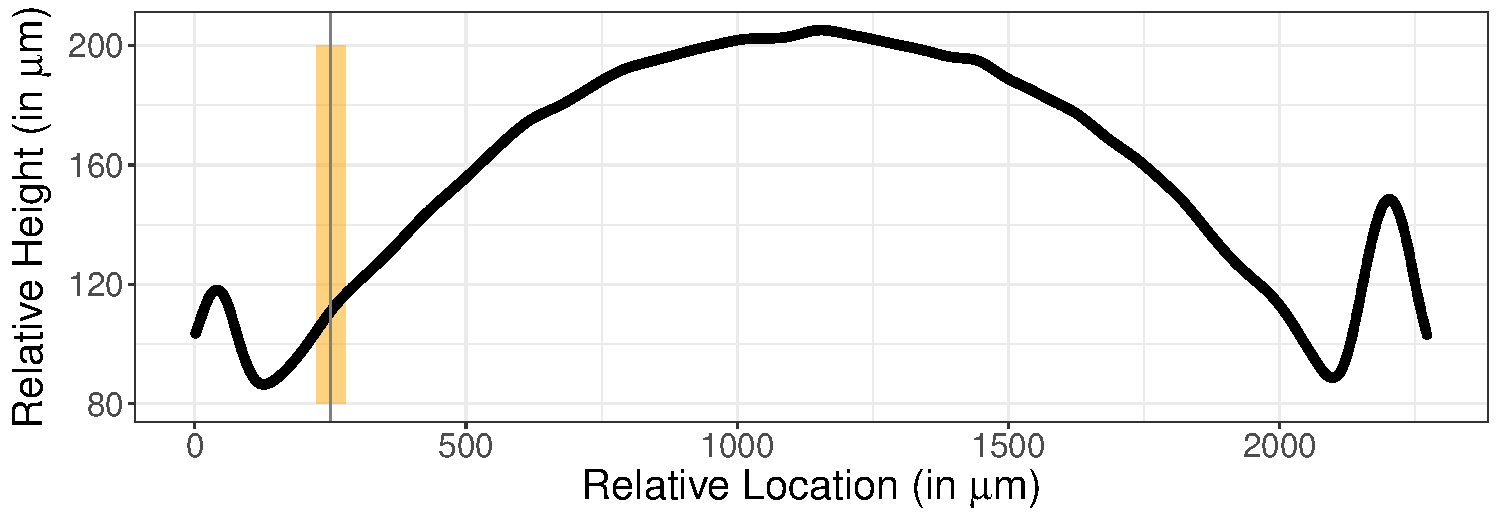
\includegraphics[width=.5\textwidth]{loess_step3-1} 

\end{knitrout}
\end{subfigure}
\begin{subfigure}[t]{\textwidth}\centering
\caption{\label{fig:loess_step47}Steps 3 -- 6 of identifying groove locations: After smoothing the surface measurements extrema on the left and right are detected (marked by vertical lines, red indicating peaks and blue indicating valleys). Values outside the blue boundaries are removed (shown in grey)}
\begin{knitrout}
\definecolor{shadecolor}{rgb}{0.969, 0.969, 0.969}\color{fgcolor}
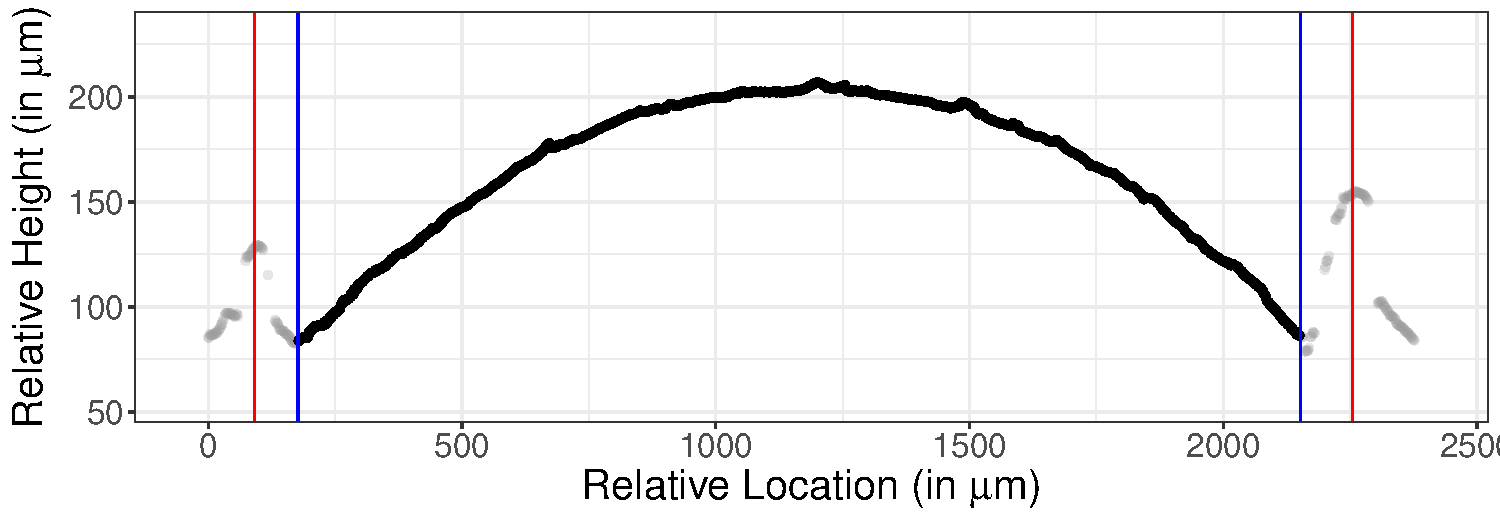
\includegraphics[width=.5\textwidth]{loess_step47-1} 

\end{knitrout}
\end{subfigure}
\caption{Overview of all six steps of the smoothing algorithm to identify and remove grooves from the bullet images.}
\end{figure}

The smoothing factor $s$ introduced in the algorithm represents the window size to use for a rolling average. Higher values of $s$ therefore lead to more smoothed results. In the groove detection portion of this algorithm, we wish to remove most of the deviation but still maintain enough signal in the groove to detect it. Empirically, a value of $s = 35$ for the smoothing factor seems to work quite well (the smoothing factor is further discussed in Section~\ref{sec:smoothing}). It is important to note that the smoothing pass is done twice. That is, the smoothed data is once again smoothed by computing a new rolling average with the same smoothing factor. This bears some similarities to the ideas of John Tukey in his book Exploratory Data Analysis, where he describes a smoothing process called ``twicing" in which a second pass is made on the residuals computed from the first pass and then added back to the result~\citep{tukey:1977}. This has the effect of introducing a bit more variance back into the smoothed data. 
We instead performed a second smoothing pass on the smoothed data, which has the effect of weighting observations near the center of the window the highest, with the weights linearly dropping off as we reach either end of the smoothing window.

\subsection{Removing curvature}
Next, we fit a loess regression to the data. Loess regression \citep{cleveland:1979} is based on the assumption that the relationship between two random variables $X$ and $Y$ can be described in form of a smooth, continuous function $f$ with $y_i = f(x_i) + \varepsilon_i$ for all values $i = 1, ..., n$. The function $f$ is approximated via locally weighted polynomial regressions. Parameters of the estimation are $\alpha$, the proportion of all points included in the fit (here, $\alpha = 0.75$), the weighting function and the degree of the polynomial (here, we fit a quadratic regression). 

The main idea of locally weighted regression is to use a weighting routine that  emphasizes the effect of points close by and de-emphasizes the effect of points as they are further away. The weighting function used here, is the tricubic function $w(d) = \left(1 - d^3\right)^3$, for $d \in [0,1]$ and $w(d) = 0$ otherwise. Here, $d$ is defined as the distance between $x_i$ and the location of the fit $x_o$ and the maximum distance of the range of the $x$-values for span $\alpha$ in $x_o$. 

%\hh{XXX standard errors: are based on independence of errors (which we don't have because of the high autocorrelation) and the assumption that the amount of bias is neglible. Which we don't know. We can produce standard errors, but (a) the nominal confidence level will be violated, and (b) the errors only allow for pointwise errors. We need a different approach. XXX}

Figure~\ref{fig:loess_fit} shows the loess fit, in blue, overlaid on the processed image of bullet~1-5. The fit seems to do a reasonable job of capturing the structure of the image. The blue area around the signature are  95\% bootstrapped confidence intervals based on 1,000 bootstrap samples. 
Figure~\ref{fig:loess_resid} shows the residuals from this fit. These residuals are called the \emph{signature} of bullet~1-5.
%
\begin{figure}[hbtp]
  \centering
\begin{subfigure}[b]{.49\textwidth}\centering
\caption{\label{fig:loess_fit} Loess fit for bullet~1-5.}
\begin{knitrout}
\definecolor{shadecolor}{rgb}{0.969, 0.969, 0.969}\color{fgcolor}
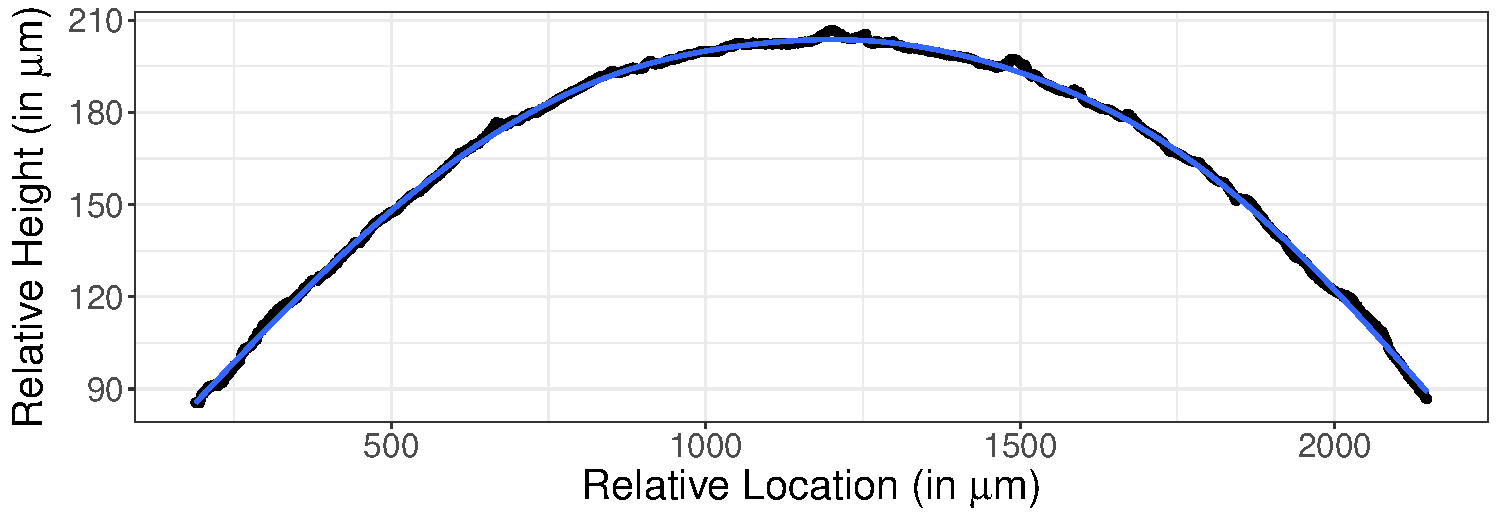
\includegraphics[width=\textwidth]{loess_fit-1} 

\end{knitrout}
\end{subfigure}
\begin{subfigure}[b]{.49\textwidth}\centering
\caption{\label{fig:loess_resid} Residuals of loess fit for bullet~1-5.
}
%<<loess_resid, echo=FALSE, fig.width=10, fig.height=3.5, out.width='\\textwidth', warning=FALSE>>=
%my.loess$resid + ylab("Residuals of loess Fit") 
%@
\begin{knitrout}
\definecolor{shadecolor}{rgb}{0.969, 0.969, 0.969}\color{fgcolor}
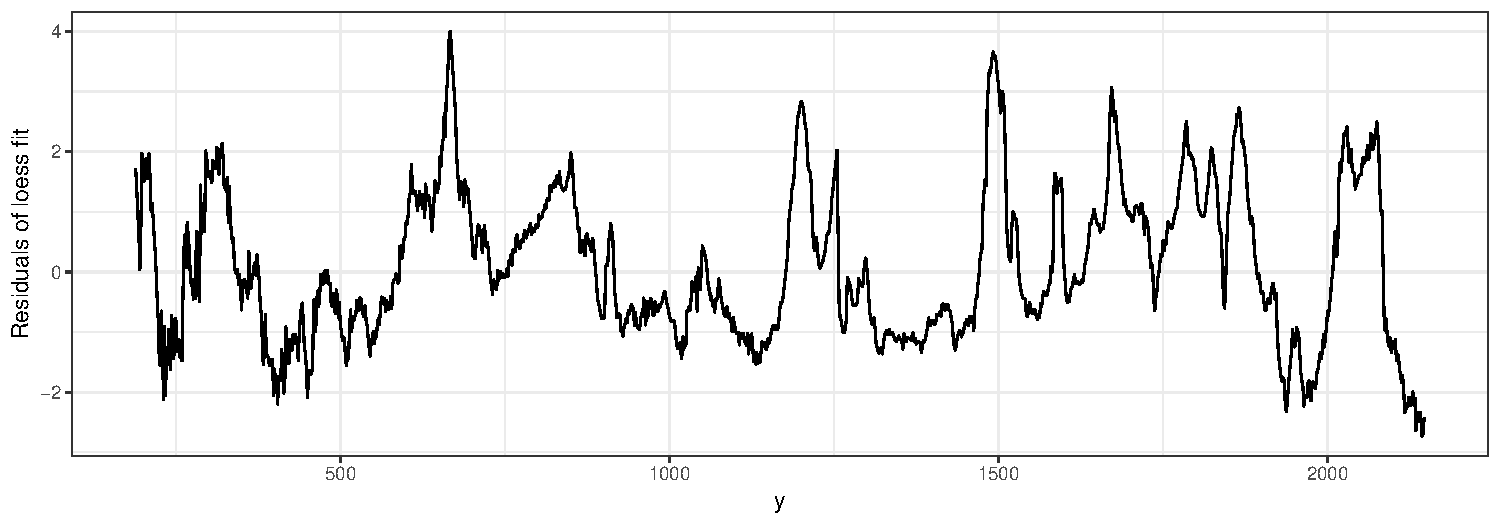
\includegraphics[width=\textwidth]{boot_loess-1} 

\end{knitrout}
\end{subfigure}
\caption{Fit and residuals of a loess fit to bullet~1-5 (Barrel~1). The residuals define the {\it signature} of bullet~1-5. Blue areas around the residuals show  95\% bootstrap confidence intervals (based on $B=1,000$ bootstrap samples).
}
\end{figure}
%

%' \hh{XXX Do we need the next example? We could save some space here XXX}
%' Figure~\ref{fig:loessfits} shows the signatures of all lands of bullet 2 (in grey) fired from the same barrel as bullet~1. The darker line overlaid on each of the signatures, shows signature from bullet~1-5. 
%' %We can reproduce a similar figure to the one from the circular fits by overlaying the residuals from each loess fit for bullet 2 onto an image of the loess residuals from bullet~1-5. This is shown in Figure~\ref{fig:loessfits}. 
%' Bullet 2-1 is the best match for bullet~1-5, but the alignment is not quite  correct. \hh{This is one of the issues we are addressing next.}
%' 
%' \begin{figure}[hbtp]
%'   \centering
%' <<loessfits, echo=FALSE, fig.width=10, fig.height=5, out.width='\\textwidth', warning=FALSE>>=
%' br121.groove <- get_grooves(br121_bullet)
%' br122.groove <- get_grooves(br122_bullet)
%' br123.groove <- get_grooves(br123_bullet)
%' br124.groove <- get_grooves(br124_bullet)
%' br125.groove <- get_grooves(br125_bullet)
%' br126.groove <- get_grooves(br126_bullet)
%' 
%' my.loess1 <- fit_loess(br121_bullet, br121.groove)
%' my.loess2 <- fit_loess(br122_bullet, br122.groove)
%' my.loess3 <- fit_loess(br123_bullet, br123.groove)
%' my.loess4 <- fit_loess(br124_bullet, br124.groove)
%' my.loess5 <- fit_loess(br125_bullet, br125.groove)
%' my.loess6 <- fit_loess(br126_bullet, br126.groove)
%' 
%' my.loessactual <- fit_loess(br111_bullet, br111.groove)
%' 
%' minrows <- min(length(my.loess1$data$resid),
%'                length(my.loess2$data$resid),
%'                length(my.loess3$data$resid),
%'                length(my.loess4$data$resid),
%'                length(my.loess5$data$resid),
%'                length(my.loess6$data$resid),
%'                length(my.loessactual$data$resid))
%' 
%' my.df <- data.frame(y = my.loess1$data$y[1:minrows], resid1 = my.loess1$data$resid[1:minrows],
%'                     resid2 = my.loess2$data$resid[1:minrows], resid3 = my.loess3$data$resid[1:minrows],
%'                     resid4 = my.loess4$data$resid[1:minrows], resid5 = my.loess5$data$resid[1:minrows],
%'                     resid6 = my.loess6$data$resid[1:minrows])
%' 
%' melt.df <- my.df %>%
%'     gather(key = part, value = resid, resid1:resid6)
%' melt.df$part <- gsub("resid", "", melt.df$part)
%' 
%' actual.df <- my.loessactual$data[1:minrows,]
%' melt.df$land <- melt.df$part
%' qplot(y, resid, data=melt.df, #colour=factor(x), 
%'       geom="line", size=I(.75), colour=I("grey70")) + 
%'   facet_wrap(~land, ncol=3, labeller="label_both") + 
%'   scale_colour_brewer(palette="Paired") +
%'   theme_bw() + theme(legend.position="bottom") + 
%'   geom_line(data = actual.df, aes(y, resid), colour="black", size=.75, alpha=0.5) + ggtitle("Signatures of bullet 1 in grey, bullet 1-5 in black") + 
%'   ylab("Residuals of loess fit") +
%'   theme(plot.margin = unit(c(0,0,0,0), unit="cm"))
%' @    
%' \caption{\label{fig:loessfits} Residuals of a loess fit to bullets 1 and 2 from barrel 1. Bullet~1-5 is shown in black. }
%' \end{figure}
%' 

\section{Automatic matching}
Applying the loess fit to a range of different signatures (see Figure~\ref{fig:manualmatch-rgl} for signatures extracted at heights between 50$\mu m$ and 150~$\mu m$) shows the 3D striation marks from two bullets. Signatures of bullet~1 are shown on the left (all extracted from heights below 100$\mu m$) and signatures of bullets 2 are shown on the right (extracted at heights above 100$\mu m$). Signatures are manually aligned, resulting in many of the striation marks to continuously pass from one side to the other. Visually, this allows for an easy assessment of these two bullet lands as a match. However, this match relies on visual inspection and can therefore not be completely objective.  The goal of this section is to eliminate the need for a visual inspection during the matching process and replace it by an automatic algorithm. This also allows for a quantification of the quality of the match.

\begin{figure}[hbtp]
\centering
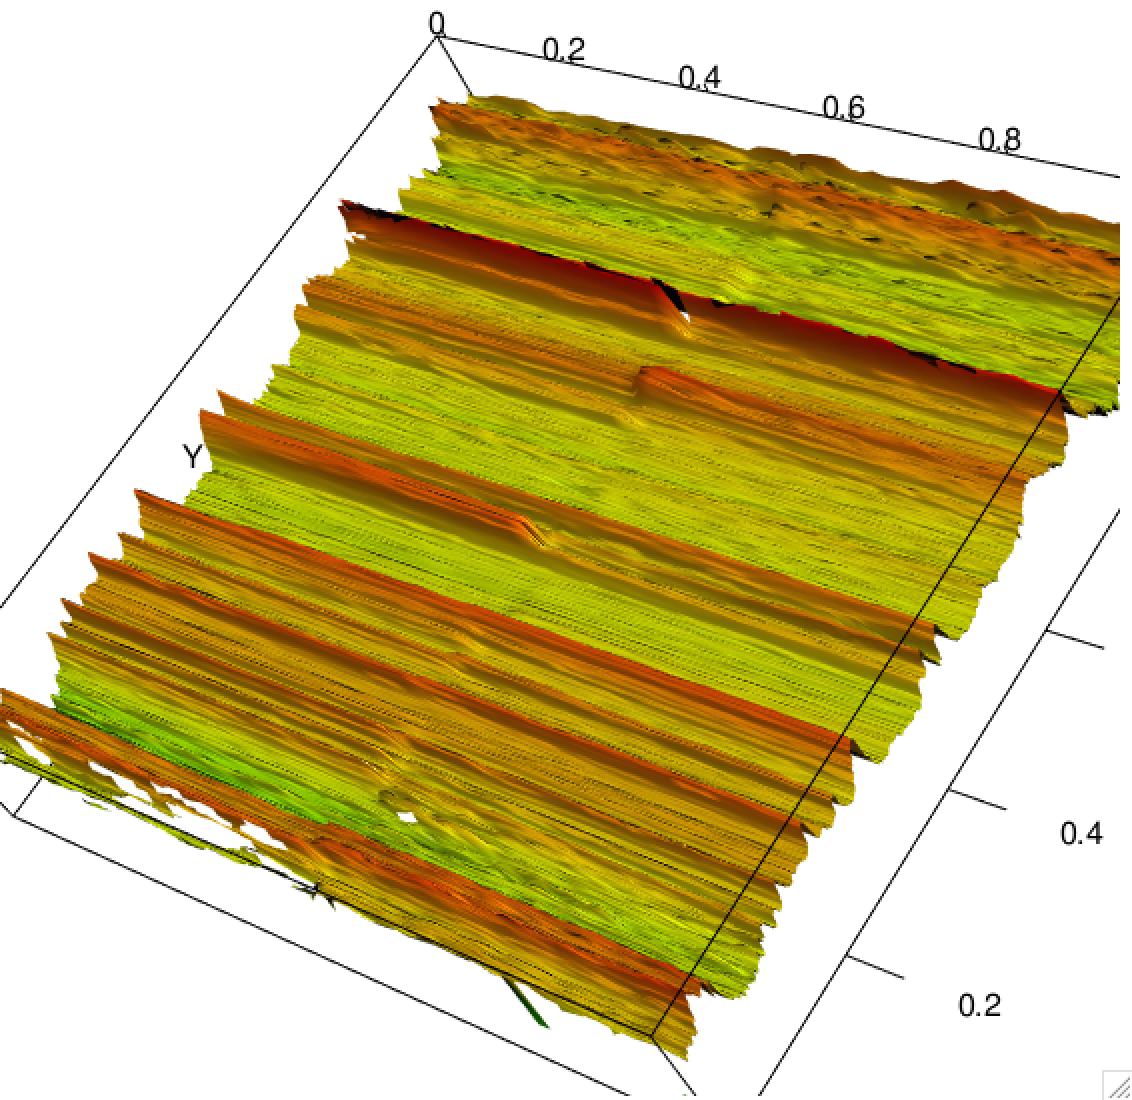
\includegraphics[width=.65\columnwidth]{matchup-rgl.png}
\caption{\label{fig:manualmatch-rgl}3D view of the manually adjusted side-by-side comparison of bullet~1-5 and bullet 2-1 after removing the curvature.}
\end{figure}

In this section, we describe the algorithm for matching signatures first, and the impact of parameter choices in the subsections thereafter.


\subsection{Algorithm}\label{sec:algorithm}






\begin{figure}[hbtp]
\centering
    \begin{subfigure}[t]{\textwidth}\centering
\caption{Loess smooth of signatures  at a height of $x = 100\mu m$ (span is 0.03).\label{fig:smooth}}{%
\begin{knitrout}
\definecolor{shadecolor}{rgb}{0.969, 0.969, 0.969}\color{fgcolor}
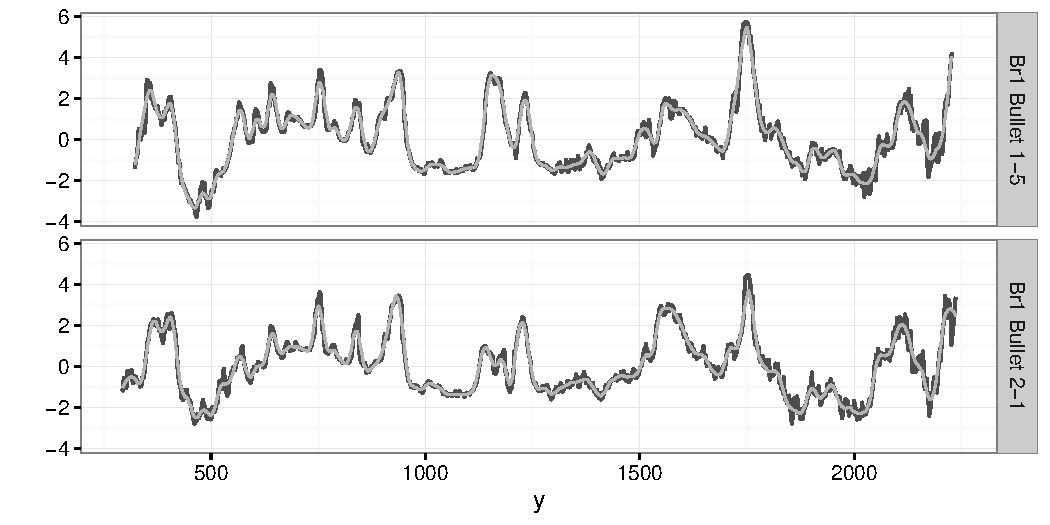
\includegraphics[width=.65\textwidth]{smooth-1} 

\end{knitrout}
    }
\end{subfigure}
\begin{subfigure}[t]{\textwidth}\centering
\caption{Using a rolling median peaks and valleys are identified for each signature. Peaks and valleys on the signature correspond to striation marks on the bullet's surface. \label{fig:smoothcutb}}{%
\begin{knitrout}
\definecolor{shadecolor}{rgb}{0.969, 0.969, 0.969}\color{fgcolor}
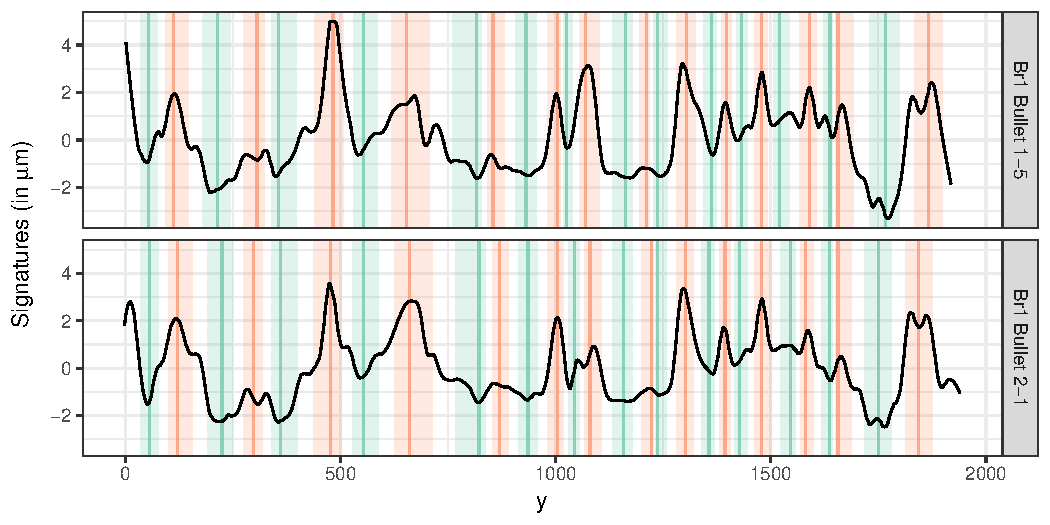
\includegraphics[width=.65\textwidth]{smoothcut-1} 

\end{knitrout}
}
\end{subfigure}    
\begin{subfigure}[t]{\textwidth}\centering
    \caption{Rectangles in the back identify a striation mark on one of the bullets.  Matching striation marks are indicated by color filled rectangles and marked by an `o'. Mismatches are filled in grey and  marked by an `x'.   \label{fig:smoothcutd}}{%
\begin{knitrout}
\definecolor{shadecolor}{rgb}{0.969, 0.969, 0.969}\color{fgcolor}
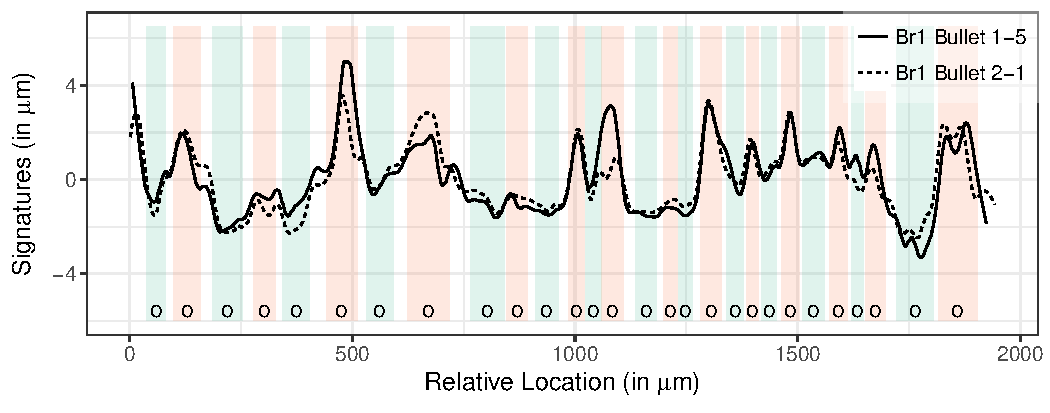
\includegraphics[width=.65\textwidth]{smoothmatch-1} 

\end{knitrout}
    }
\end{subfigure}
\caption{\label{fig:match}Matching striation marks: smooth (a), identify peaks and valley (b), and match peaks and valleys between signatures (c).}
\end{figure}
%\afterpage{\clearpage}
Figure~\ref{fig:match} gives an overview of the automated matching routine: 
We first identify a stable region for each bullet land and extract the signature at the lowest height in this region, because typically, individual characteristics are best expressed at the lower end of the bullet (see Supplement section~\ref{supp:bulletbottom} for a more detailed discussion). 

All of the other steps are done on pairs of bullet lands:
\begin{enumerate}
\item {\bf Smooth the two signatures} by a loess with a very small span (see Figure~\ref{fig:smooth}). 
\item Use cross-correlation to {\bf find the best alignment} of the two signatures: shift one of the signatures by the lag indicated by the cross-correlation function (see Figure~\ref{fig:ccf} for the cross-correlation function and Figure~\ref{fig:crosscutX} for the resulting shift).
\item Using a rolling average, {\bf identify peaks and valleys} for each of the signatures. We then define an interval around the location of the extrema on each side as one third of the distance to the location of the next extrema (see Figure~\ref{fig:smoothcutb}). Peaks and valleys constitute the \emph{striation marks} of the bullet.
\item {\bf Match striations across signatures:} based on the intervals around the extrema as defined above, we identify joint intervals between two signatures as those areas, in which two or more of the individual intervals overlap: a joint interval is defined as the smallest interval that encompasses all of the overlapping intervals. A joint interval is then called a match(ing stria) between the signatures, if all of the intervals are of the same type of extrema, i.e.\ they are either all peaks or all valleys. In Figure~\ref{fig:match} all matches are shown as color-filled rectangles corresponding to their type of extrema (peaks are shown in orange, and valleys in green). Non-matching intervals are left grey. 
\item {\bf Extract features from the aligned signatures and the matches between them:} many different features could be extracted. Here, we describe a few of the ones that can be found in the literature and some that we found to be of practical relevance:
\begin{enumerate}[label=(\roman*)]
\item Maximal number of CMS (consecutive matching striae), and, similarly, the number of consecutively non-matching striae (CNMS), 
\item Number of matches and non-matches,
\item Average difference $D$ between signatures, defined as the Euclidean vertical distance between surface measurements of aligned signatures. Let $f(t)$ and $g(t)$ be smoothed, aligned signatures:
\[
D^2 = \frac{1}{\text{\#}t}\sum_t \left[f(t) - g(t)\right]^2,
\]
\item The sum $S$ of average absolute heights of matched extrema: for each of the two matched stria, compute the average of the absolute heights of the peaks or valleys. $S$ is then defined as the sum of all these averages. 
\end{enumerate}
\end{enumerate}
%
The difference $D$ between signatures is here defined as the Euclidean distance (in $\mu m$). In the paper by \citet{ma:2004}, distance is defined as a measure relative to the first signature, which serves as a comparison reference and is therefore a unitless quantity. 

Counting the maximal number of CMS is part of current practice to identify bullet matches~\citep{nichols:1997, nichols:2003, nichols:2003b}. 
In the example of Figure~\ref{fig:match}, the number of consecutive matching striations (CMS) is fifteen, a  high number indicative of a match between the bullets. 
 Note that the definition of CMS given in this paper does not match the one given in \citet{thompson:2013}. There, CMS is defined only in terms of matching peaks without regarding valleys. Additionally, peaks in  \citet{thompson:2013} are  used only if they can be identified and matched `within a tolerable range' between lands. The definition given here is computationally less complex, but should yield highly correlated values, because of the requirement to only consider signatures from a stable region in the land (see Section~\ref{sec:heights} for further details on stability of regions). In the Hamby study, the definition of CMS by \citet{thompson:2013} leads to approximately half of the values of CMS defined in this paper (with a correlation coefficient between the values of the two definitions of about 0.92). 
For lead bullets, such as used in the Hamby study, \citet{biasotti:1959} considered four or more consecutive peaks (corresponding to eight or more consecutive lines in our definition) to be sufficient evidence of a match.  %We will assess the claim that eight or more consecutive lines are sufficient for a match in the next section. 

Determining a threshold such that CMS values above the threshold indicate a match with high reliability is beyond the scope of this work, even though it is critically important in practice. We provide some ideas in the next section, but first we assess the robustness of the matching algorithm to different choices of the parameter values. 
%In order to get a better understanding of  how  this matching works in known matches and non-matches, we next investigate the algorithm's performance in a test scenario.
In addition to the features listed above, we also keep track of the value of the cross-correlation function found during the alignment, the lag at which signatures show the best alignment, and the height at which signatures are extracted ($x_1$ and $x_2$).

%' \begin{figure}[hbtp]
%'   \centering
%' <<barrel2, echo=FALSE, fig.width = 10, fig.height=6, out.width='\\textwidth', warning=FALSE>>=
%' 
%' list_of_matches <- lapply(25:30, function(i) {
%'   lof <- processBullets(paths = images[c(31,i)], x = 100)
%'   lof <- bulletSmooth(lof)
%' 
%'   bAlign = bulletAlign(lof)
%'   lofX <- bAlign$bullet  
%' 
%'   b12 <- unique(lof$bullet)
%'   peaks1 <- get_peaks(subset(lofX, bullet==b12[1]), smoothfactor = 25)
%'   peaks2 <- get_peaks(subset(lofX, bullet == b12[2]), smoothfactor = 25)
%'   peaks1$lines$bullet = b12[1]
%'   peaks2$lines$bullet = b12[2]
%'   lines <- striation_identifyXXX(peaks1$lines, peaks2$lines)
%' 
%'   ggplot() +
%'     theme_bw() + 
%'     geom_rect(aes(xmin=xmin, xmax=xmax, fill=factor(type)), show.legend=FALSE, ymin=-6, ymax=6, data=lines, alpha=0.2) +
%'     geom_line(aes(x = y, y = l30, linetype = bullet),  data = lofX, alpha=0.6) +
%'     scale_linetype_discrete("") +
%'     scale_fill_brewer("", palette="Set2", na.value=alpha("grey50", alpha=0.5)) +
%'   theme(legend.position = c(1,1.2), legend.justification=c(1,1),
%'         legend.background = element_rect(fill=alpha('white', 0.4))) + 
%'     ylim(c(-6,6)) + ylab("") + xlab("") +
%'     geom_text(aes(x = meany), y= -5.5, label= "x", data = subset(lines, !match)) +
%'     geom_text(aes(x = meany), y= -5.5, label= "o", data = subset(lines, match)) +
%' #    theme(plot.margin=unit(c(1,0,0,0), unit="line")) +
%'     theme(plot.margin=unit(c(0,0,0,0), unit="cm"))
%' })
%' 
%' grid.arrange(list_of_matches[[1]], list_of_matches[[2]], list_of_matches[[3]], 
%'              list_of_matches[[4]], list_of_matches[[5]], list_of_matches[[6]],
%'              ncol = 2)
%' @
%' \caption{\label{fig:barrel2}All lands from the first bullet shot from barrel 2 are compared to Bullet 2-1 (barrel 2). The largest number of CMS is eleven, observed with Bullet 1-6. \hh{XXX Do we need this example? This might be a place to cut XXX}}
%' \end{figure}

\subsection{Horizontal alignment}
Signatures of each of the two lands, 1-5 and 2-1,  in Figure~\ref{fig:manualmatch-rgl} are shown in Figure~\ref{fig:cross100} extracted at a height of $x = 100\mu m$. Striation marks show up in this representations as peaks and valleys.  The individual characteristics are quite prominent and, again, suggest a match between the lands. A horizontal shift of one of the signatures (result shown in Fig~\ref{fig:crosscutX}) emphasizes the strong similarities. 
%
\begin{figure}[hbtp]
\centering
\begin{subfigure}[b]{.49\textwidth}\centering
\caption{Raw bullet land signatures.\label{fig:crosscut}}{%
\begin{knitrout}
\definecolor{shadecolor}{rgb}{0.969, 0.969, 0.969}\color{fgcolor}
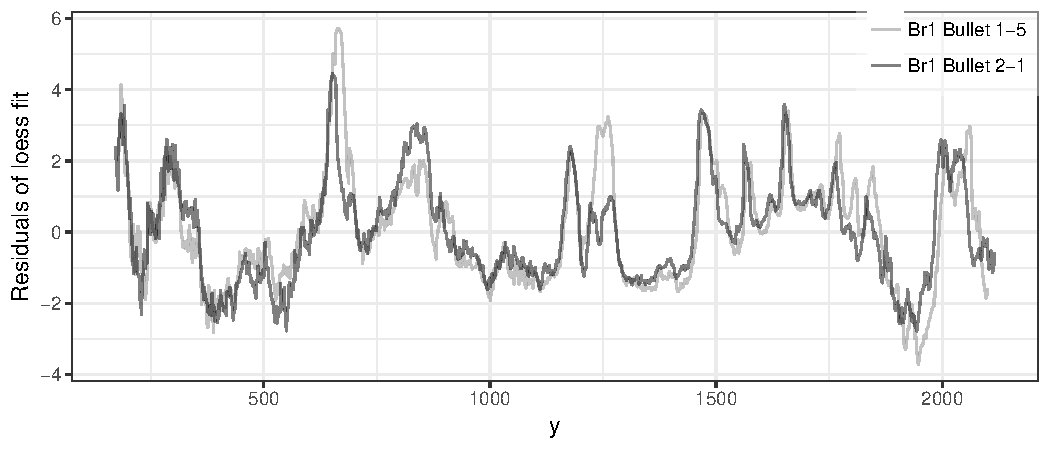
\includegraphics[width=\textwidth]{crosscuts-1} 

\end{knitrout}
    }
\end{subfigure}    
\begin{subfigure}[b]{.49\textwidth}\centering
    \caption{Aligned signatures.\label{fig:crosscutX}}{%
\begin{knitrout}
\definecolor{shadecolor}{rgb}{0.969, 0.969, 0.969}\color{fgcolor}
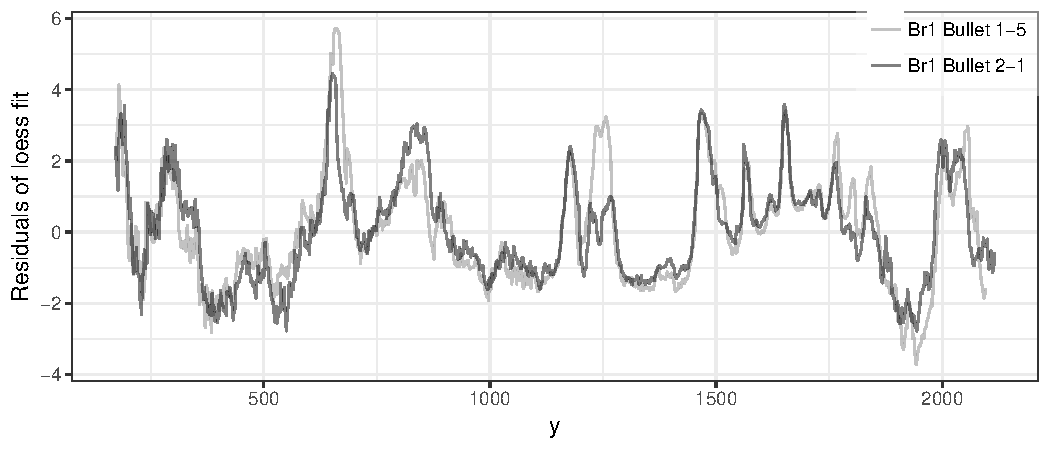
\includegraphics[width=\textwidth]{crosscutsX-1} 

\end{knitrout}
    }
\end{subfigure}
\caption{\label{fig:cross100}Signatures of bullets 1-5 and 2-1 taken at  heights of $x = 100\mu m$. A horizontal shift of the values of bullet~1-5 to the right shows the similarity of the striation marks.}
\end{figure}
%
This horizontal shift is based on the cross-correlation between the two signatures: let $f(t)$ and $g(t)$ define the signature values  at $t$, where $t$ are locations between 0~$\mu m$ and about 2500~$\mu m$, 1.5625~$\mu m$ apart.
The cross-correlation between $f$ and $g$ at lag $k$ is then defined as
\[
(f * g) (k) = \sum_t f(t+k) g(t),
\]
with suitably defined limits for the summation. % (because variances of $f$ and $g$ do not change, the above equation is proportional to the correlation). 

\begin{figure}[hbtp]
  \centering
\begin{knitrout}
\definecolor{shadecolor}{rgb}{0.969, 0.969, 0.969}\color{fgcolor}
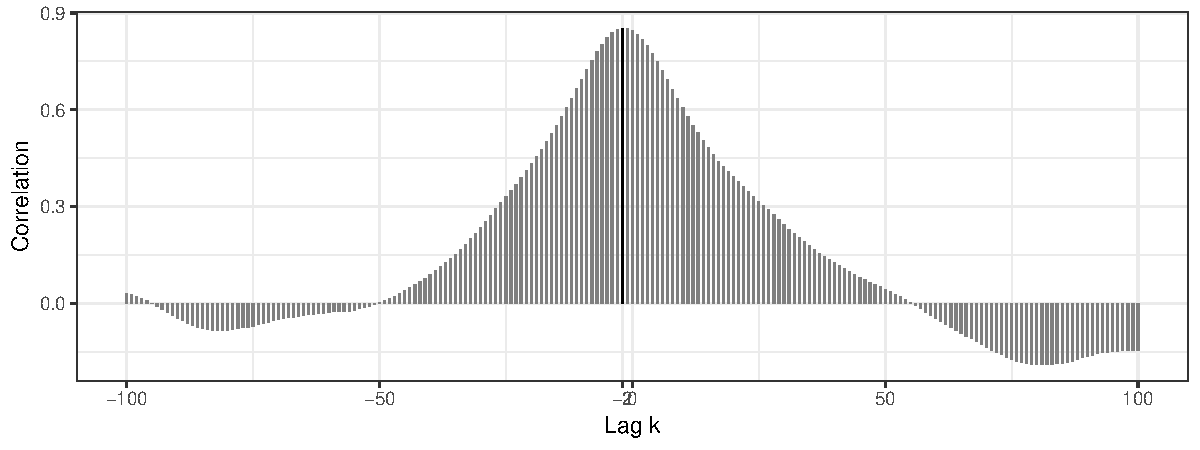
\includegraphics[width=.65\textwidth]{ccf-1} 

\end{knitrout}
\caption{\label{fig:ccf}Cross-correlation function between the two signatures shown in Figure~\ref{fig:crosscut} at lags between -100 and 100. At a lag of -17 the correlation peaks, indicating the largest amount of agreement between the signatures. Figure~\ref{fig:crosscutX} shows the lag-shifted signatures.}
\end{figure}


\subsection{Impact of bullet height}\label{sec:heights}
The height at which signatures are extracted for a comparison between bullet lands matters -- signatures taken from heights that are further apart, show more pronounced differences between the signatures. 
This poses both a caveat to matching attempts as well as an opportunity for quality control: we have to be aware of the height that was used in a matching. Visually, matches degrade if the signatures upon which the match is based are from heights further than 200$\mu m$ apart  (see Supplement section~\ref{supp:ccf} for a more thorough discussion).
However, we can extract signatures from multiple heights of the same bullet land for an initial assessment of its quality. 
This situation is assessed and discussed in more detail below: 

\begin{figure}[hbtp]
  \centering
\begin{knitrout}
\definecolor{shadecolor}{rgb}{0.969, 0.969, 0.969}\color{fgcolor}
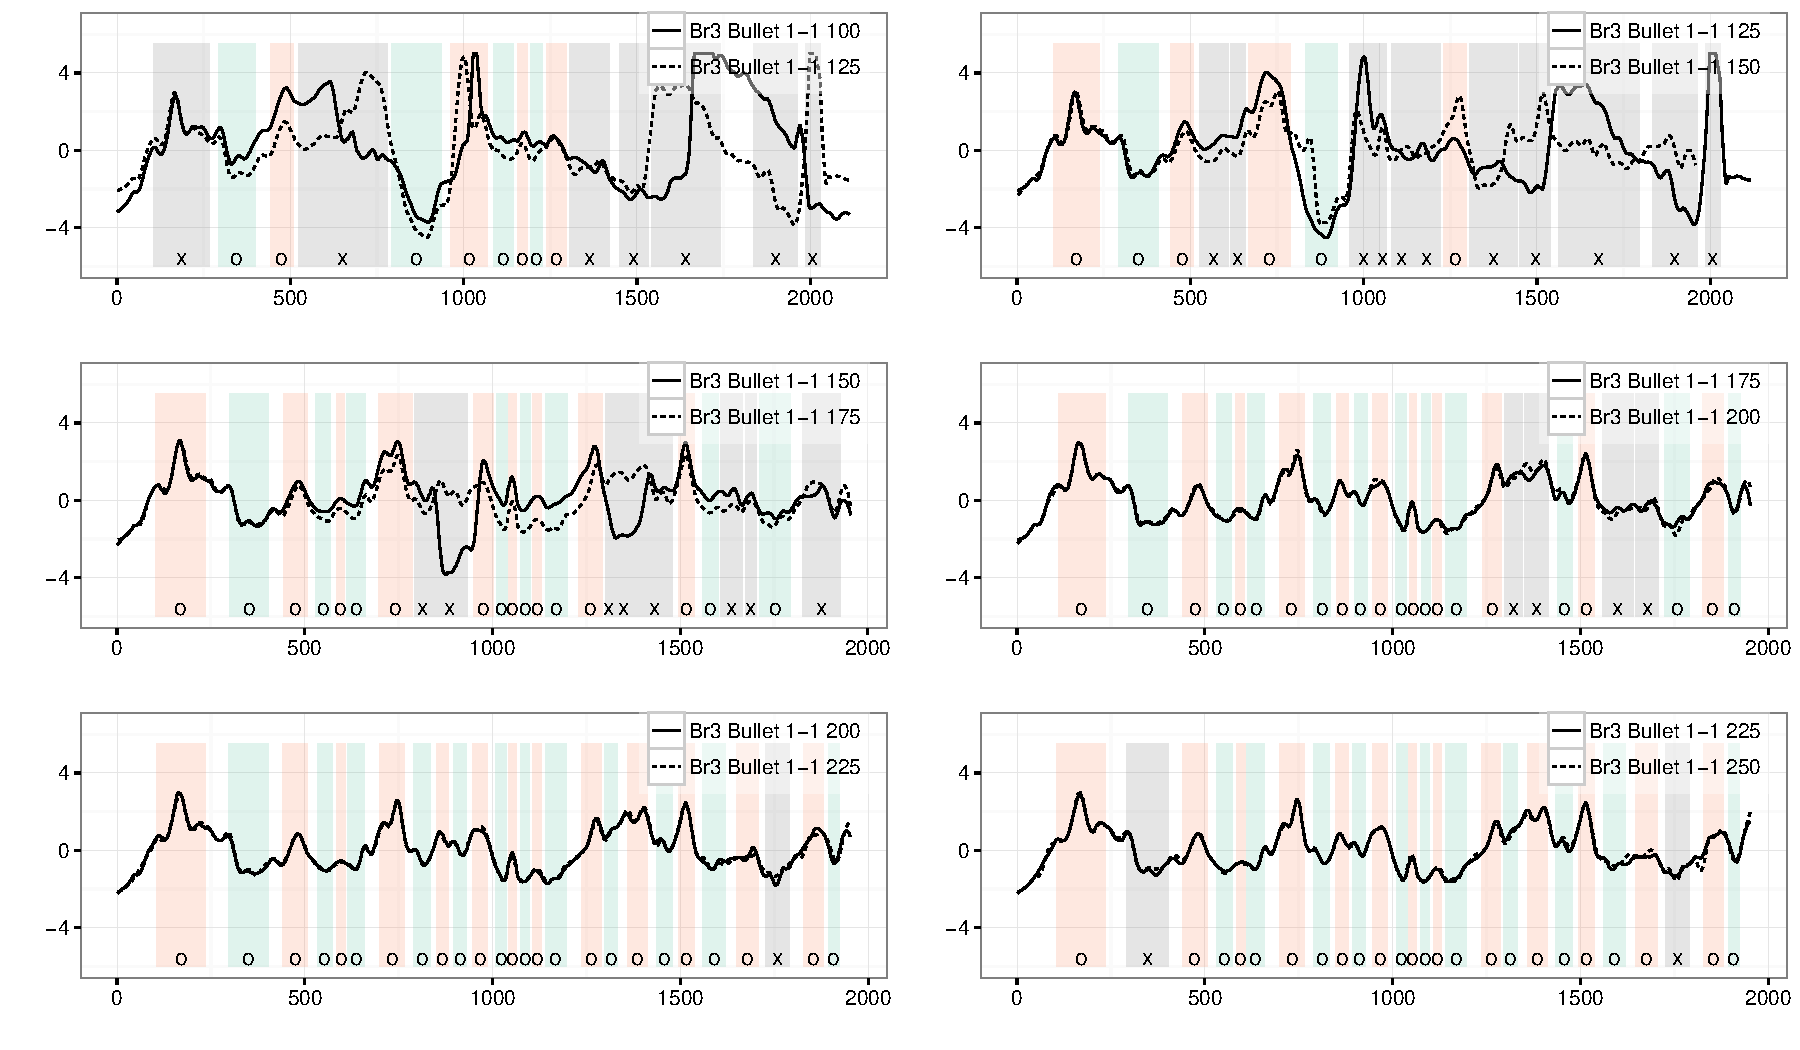
\includegraphics[width=\textwidth]{crosscuts-vary-b31-1} 

\end{knitrout}
\caption{\label{fig:crosscuts2}Signatures  for barrel 3, bullet~1-1 extracted from varying heights. Initially, the match between signatures taken at heights 25$\mu m$ apart is affected strongly by some break off at the bottom of the bullet. At a  level of $175\mu m$ the bullet's signature stabilizes. For this land, matches should not be attempted at lower heights. }
\end{figure}
%An opportunity that arises from comparing multiple cross sections of a bullet's surface measurements is the following:
by comparing signatures from heights that are not too far apart --  25~$\mu m$ to 50~$\mu m$ -- we get an indication whether the signatures come from a rapidly changing section of the surface, indicative of a break-off or some other damage, or from a stable section, where we have a reasonable expectation of finding matches to other signatures. In the approach here, we keep increasing the height $x$ at which the signature is taken until we find a section with a stable pattern. This process is shown in Figure~\ref{fig:crosscuts2} at the example of bullet~1-1 from barrel 3, where
`stability' is  defined as two aligned signatures from heights chosen 25$\mu m$ apart having a cross-correlation of at least 0.95. 

\subsection{Varying smoothing factor}\label{sec:smoothing}
As mentioned earlier, the algorithm for detecting peaks and valleys depends on the selection of a smoothing window, called the smoothing factor or span. A smoothing factor of $k$ means that the  $k$ closest observations to $x_o$ are considered for a fit for $x_o$. Because surface measurements are recorded at an equidistant resolution (here, of 1.5625$\mu m$), we decided to only consider odd smoothing factors $2k + 1$, which means that the  $k$ observations to the left and right of $x_o$ are considered for a local fit of $x_o$. For detecting and removing the grooves prior to fitting a loess regression we selected a smoothing factor  of 35, while for detecting the peaks/valleys of the loess residuals a smoothing factor of 25 seems more appropriate. %We can investigate the performance of peak/valley detection across different smoothing factors.

Figure~\ref{fig:varysmooth} displays the  peaks and valleys detected in the same signature at smoothing factors of 5, 25, and 45, respectively. The dark line corresponds to the smoothed values, while the grey line in the back shows the raw signature. The choice of smoothing factor is a classical decision of a bias/variance trade-off. It is immediately clear that a small smoothing factor like 5 is a poor choice. It results in a significant amount of noise in the data such that even just a point or two can skew the rolling average enough for a peak or valley to be detected. Given that the striation patterns are typically much larger, we are in effect muddying the waters by performing such minimal smoothing. Another consideration is that the smoothing should not fall below the  resolution of the equipment at which the surface measurements are taken -- in order to not introduce artifacts in the analysis. 

A larger smoothing factor on the other hand (like 45), seems to be a more plausible option. Most of the peaks/valleys present which are detected by a smoothing factor of 25 are also detected at 45. However, some notable issues arise. Notice that the valley on the right hand side of the image is smoothed out, and thus not detected. On the left hand side, a double peak is detected - that might be a questionable decision - but there are several peaks in the middle, that are smoothed out, for example the peak at around $y = 750$. That is, in many cases, large windows are smoothing out some of the structure that we wish to see. Furthermore, it can be seen that the peaks/valleys are often shifted relative to their position in the original loess residuals, or in the smoothed data with smaller smoothing factors.

\begin{figure}[hbtp]
  \centering
\begin{knitrout}
\definecolor{shadecolor}{rgb}{0.969, 0.969, 0.969}\color{fgcolor}
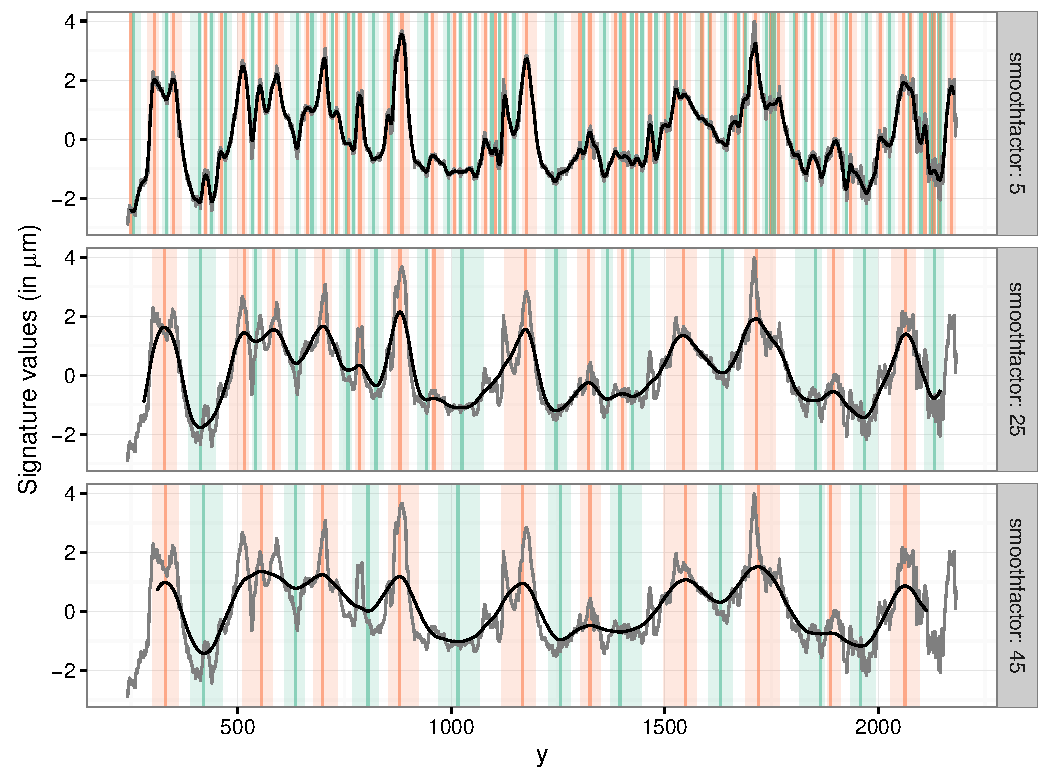
\includegraphics[width=.5\textwidth]{smoothfac1-1} 

\end{knitrout}
\caption{\label{fig:varysmooth} Peak/valley detection at smoothing factors of 5, 25, and 45, respectively. Note that a smoothing factor of 5 yields enough noise that many very minimal overlapping peaks and valleys are detected, while a smoothing factor of 45 might over-smooth and cause the peaks/valleys to either end disappear or shift  horizontally  from their position in the signature.}
\end{figure}



\section{Evaluation}
In order to get a better understanding of  how  the matching algorithm works in known matches and non-matches, we investigate its performance in a test scenario based on the James Hamby study.
As a first step, we automatically assess the quality of each of the lands by  checking that we can identify a stable region on each land. For this, we compute the cross-correlation of signatures extracted from heights 25$\mu m$ apart. For a stable region, we require a minimum of 0.95 for the cross correlation. Four lands from different bullets are flagged as problematic in this respect. A visual inspection (see Figure~\ref{fig:fourflags}) shows that each one of these lands has scratch marks across the surface, also known as `tank rash'.
%
\begin{figure}
  \centering
\begin{subfigure}[t]{.49\textwidth}\centering
\caption{Barrel 6 Bullet 2-1}
%' <<echo=FALSE>>=
%' b1 <- read.x3p(file.path(datadir, "Br6 Bullet 2-1.x3p"))
%' image(b1$surface.matrix)
%' @
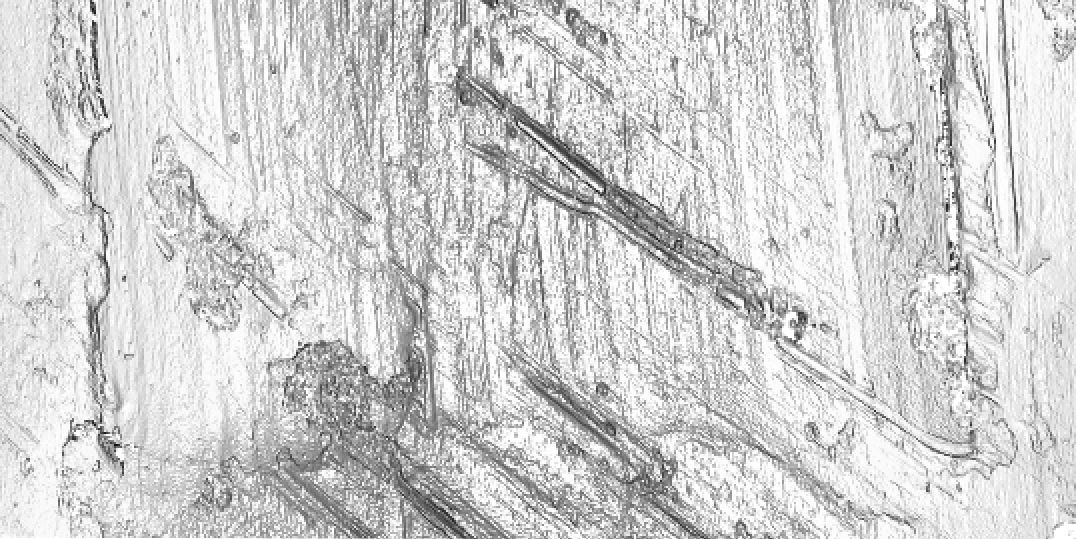
\includegraphics[width=\textwidth]{br6-2-1-grey.png}
\end{subfigure}
\begin{subfigure}[t]{.49\textwidth}\centering
\caption{Barrel 9 Bullet 2-4}
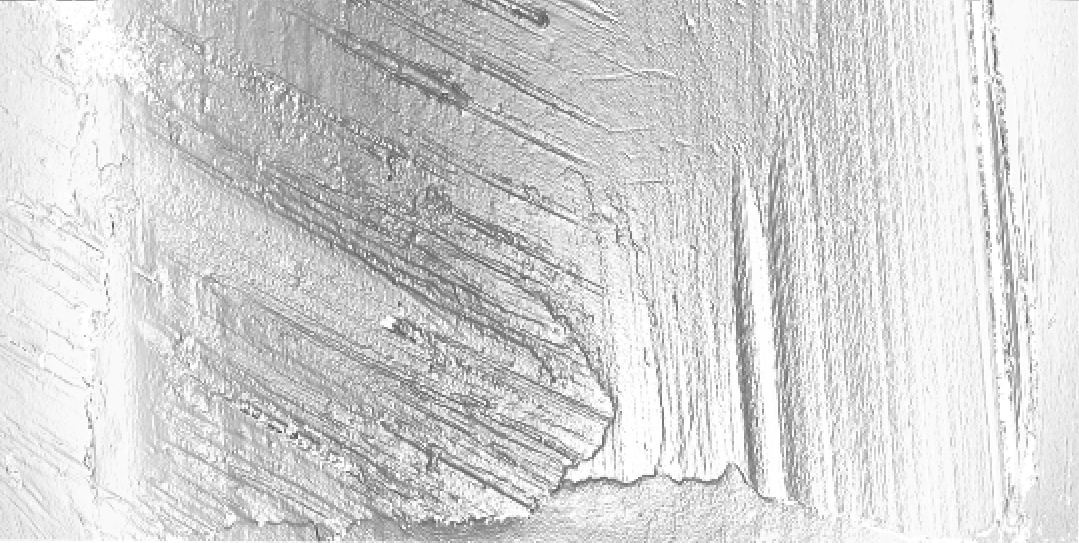
\includegraphics[width=\textwidth]{br9-2-4-grey.png}
\end{subfigure}
\begin{subfigure}[t]{.49\textwidth}\centering
\caption{Unknown Bullet B-2}
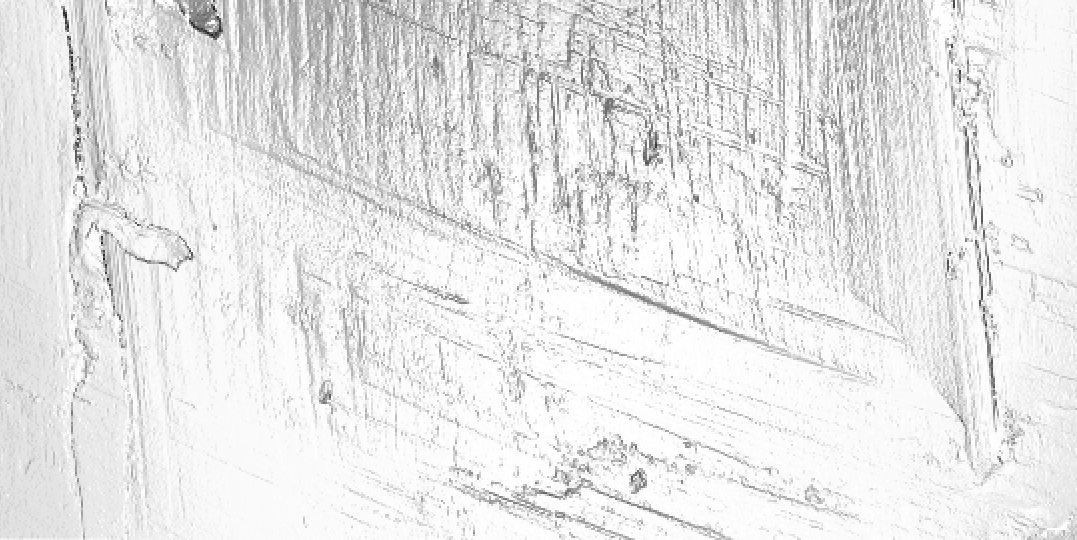
\includegraphics[width=\textwidth]{b-2-grey.png}
\end{subfigure}
\begin{subfigure}[t]{.49\textwidth}\centering
\caption{Unknown Bullet Q-4}
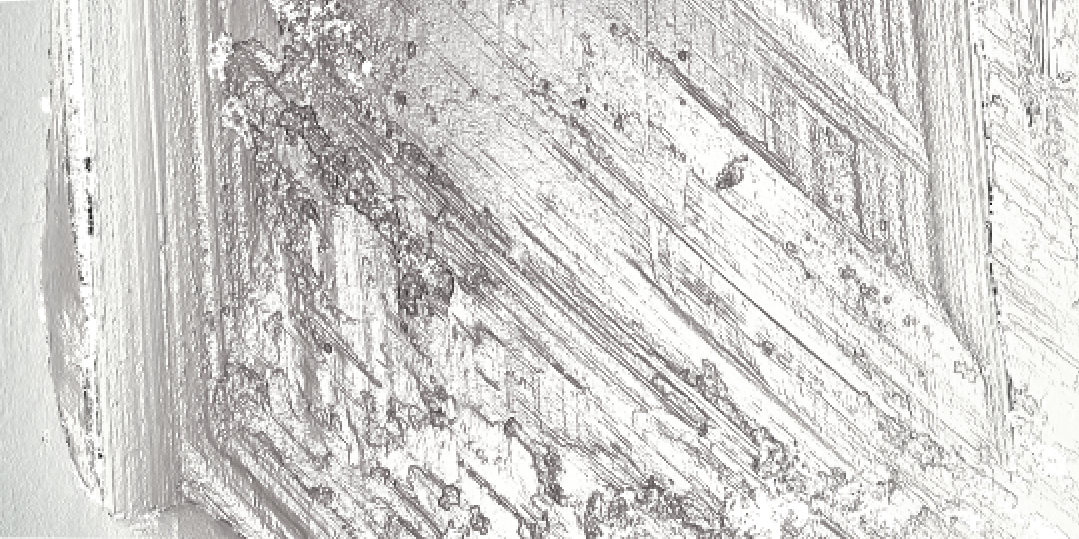
\includegraphics[width=\textwidth]{q-4-grey.png}
\end{subfigure}
\caption{\label{fig:fourflags}Images of the four lands that got flagged during the quality assessment. All of them show scratch marks (tank rash) across the striation marks from the barrel. They are excluded from the remainder of the analysis.}
\end{figure}
%
We exclude these four lands from further matching considerations and
 run all remaining lands from the unknown bullets against all remaining lands from known bullets for matches, i.e. we are comparing $15 \times 6 -2 = 90 - 2 = 88$ lands from unknown bullets against $2 \times 10 \times 6 -2 = 120 - 2 = 118$ lands from known bullets, yielding a total of $10,384$ land-to-land comparisons. Out of these comparisons, there are 172 known matches (KM), while the rest are known non-matches (KNM). 
 When things go well, they look like the results in Figure~\ref{fig:hamby-perfect}: Figure~\ref{fig:hamby-perfect}a shows the distribution of the number of maximum consecutive matching striae between land C-3 and all 118 lands from known bullets. Two lands show a high CMS. These correspond to the known matches with C-3, shown in Figures~\ref{fig:hamby-perfect}b and~\ref{fig:hamby-perfect}c. 
 Unfortunately, not all results are as clear cut. 
It might not be reasonable to assume that we can match all lands, but the idea is to try to maximize the number of matches to get an overview of what we might be able to expect from an automated match. 

\begin{figure}[hbtp]
\begin{subfigure}[t]{\textwidth}\centering
\caption{Maximal number of CMS between unknown bullet C-3 and all of the other 118 considered (known) lands. For two lands the number of maximum CMS is high. }
\begin{knitrout}
\definecolor{shadecolor}{rgb}{0.969, 0.969, 0.969}\color{fgcolor}
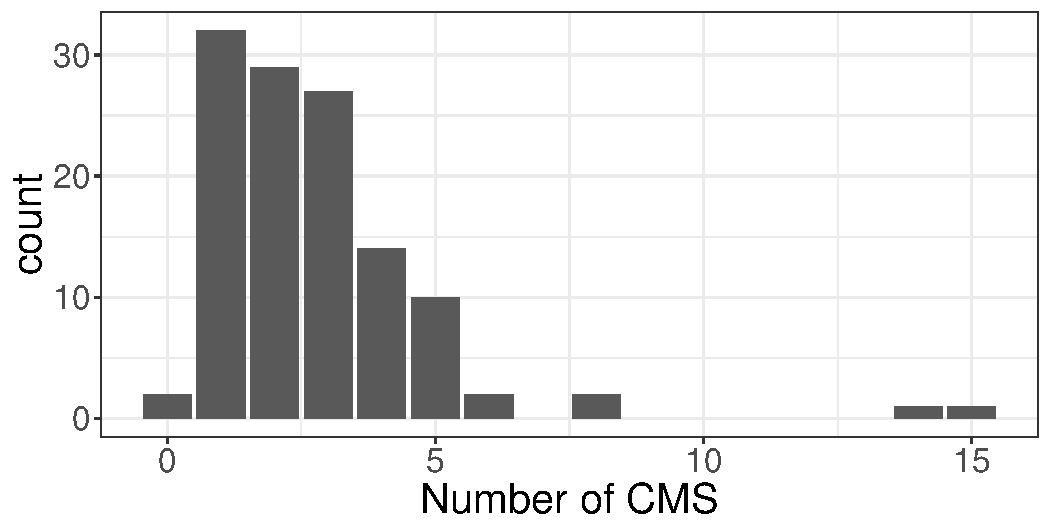
\includegraphics[width=.5\textwidth]{cms-1} 

\end{knitrout}
\end{subfigure}
\begin{subfigure}[b]{.49\textwidth}\centering
\caption{Overlaid signatures of C-3 and the land with the top matching CMS.}
\begin{knitrout}
\definecolor{shadecolor}{rgb}{0.969, 0.969, 0.969}\color{fgcolor}
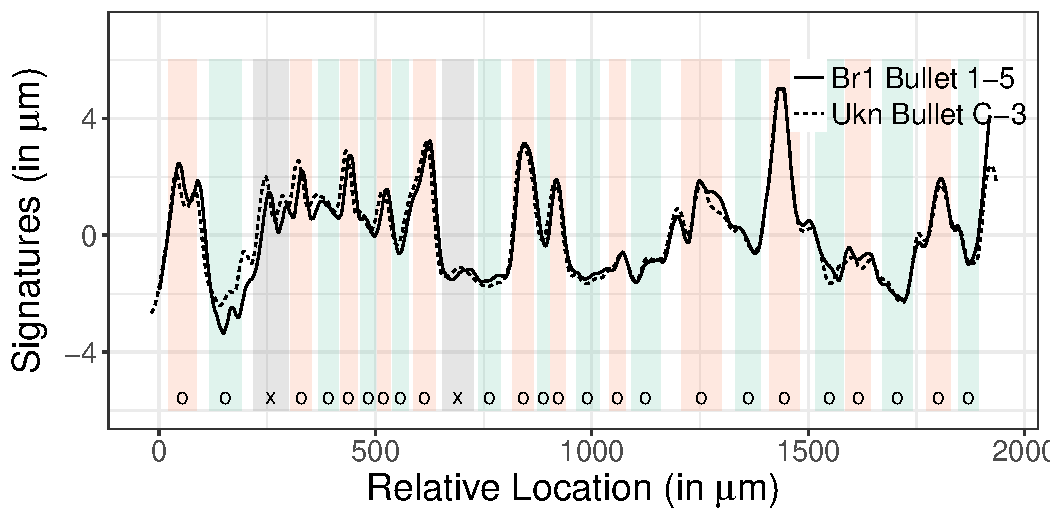
\includegraphics[width=\textwidth]{top-1} 

\end{knitrout}
\end{subfigure}
\begin{subfigure}[b]{.49\textwidth}\centering
\caption{Top 2 match with C-3 based on CMS.}
\begin{knitrout}
\definecolor{shadecolor}{rgb}{0.969, 0.969, 0.969}\color{fgcolor}
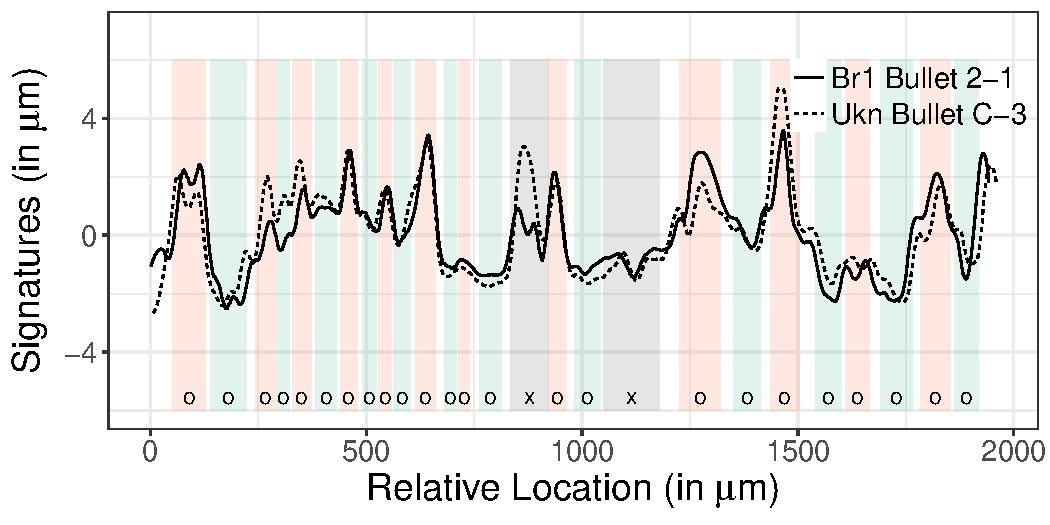
\includegraphics[width=\textwidth]{top2-1} 

\end{knitrout}
\end{subfigure}
\caption{\label{fig:hamby-perfect}Showcase scenario  when matching with CMS works very well. Unfortunately the matches are not always that convincing.}
\end{figure}

Figure~\ref{fig:cms} shows the strong connection between the maximal number of consecutive striae and matches in the Hamby study. All 42 pairs of lands with at least thirteen CMS in common are matches. 
%
\begin{figure}[hbtp]
  \centering
%' \begin{subfigure}[b]{\textwidth}\centering
%' \caption{}
\begin{minipage}[t]{.47\textwidth}
\begin{knitrout}
\definecolor{shadecolor}{rgb}{0.969, 0.969, 0.969}\color{fgcolor}
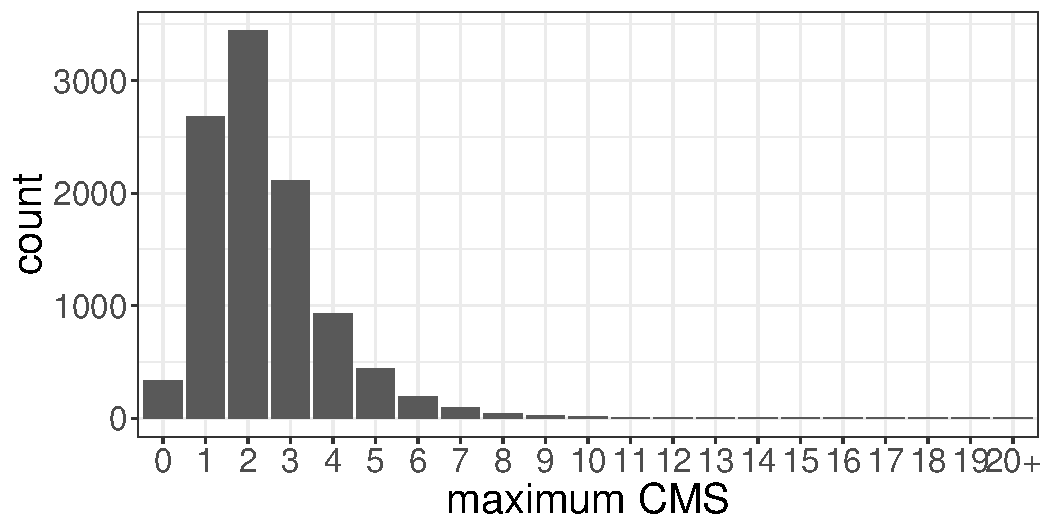
\includegraphics[width=\textwidth]{cms-bars-1} 

\end{knitrout}
%\end{subfigure}
%\begin{subfigure}[b]{\textwidth}\centering
\end{minipage}
\begin{minipage}[t]{.52\textwidth}
\begin{knitrout}
\definecolor{shadecolor}{rgb}{0.969, 0.969, 0.969}\color{fgcolor}
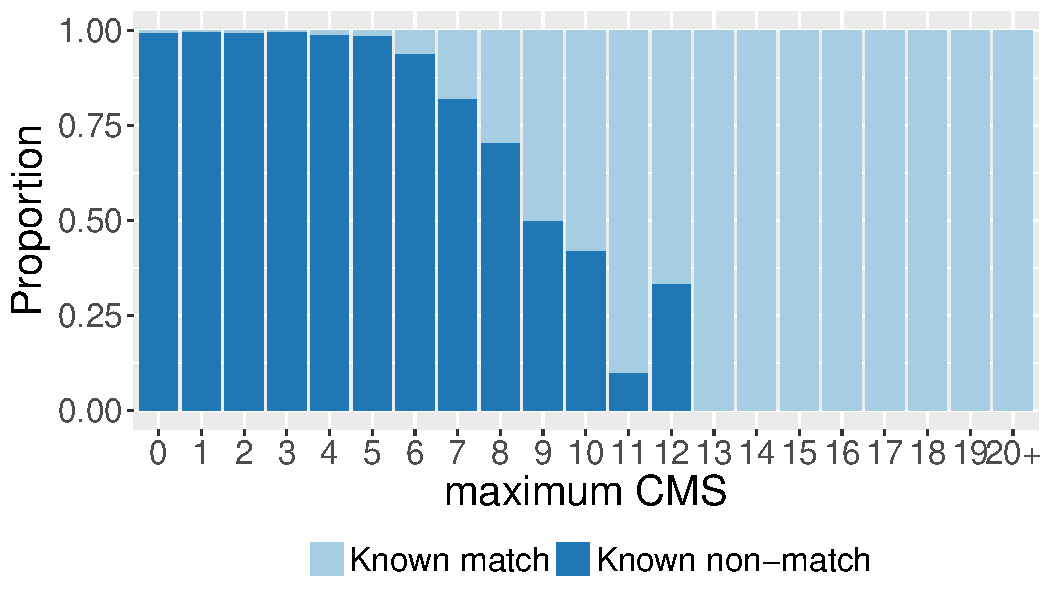
\includegraphics[width=\textwidth]{cms-spines-1} 

\end{knitrout}
\end{minipage}
%' \end{subfigure}
%' \begin{subfigure}[t]{\textwidth}\centering
%' \caption{\label{fig:cms-dens}Densities of maximum CMS for Known Matches (KM) and Known Non Matches (KNM).}
%' <<cms-densities, echo=FALSE,  fig.width=7, fig.height=3.5, out.width='.6\\textwidth'>>=
%' x <- seq(0,29, by=0.03)
%' km <- sm.density(bstats$CMS[bstats$match],h=2, model="Normal", display="none", eval.points=x)
%' knm <- sm.density(bstats$CMS[!bstats$match],h=1, display="none", eval.points=x)
%' dframe <- data.frame(x = x, km=km$estimate, knm=knm$estimate)
%' dframe$kmtail <- rev(cumsum(rev(dframe$km)))/sum(dframe$km)
%' dframe$knmtail <- rev(cumsum(rev(dframe$knm)))/sum(dframe$knm)
%' 
%' densities <- data.frame(
%'   match = rep(c("KM", "KNM"), each=(length(x)+2)),
%'   x = rep(c(0, x, 29), times = 2),
%'   estimate = c(0, km$estimate, 0, 0, knm$estimate,0))
%' 
%' ggplot() +
%'   geom_polygon(aes(x=x, y=estimate, fill=match, group=match), colour="black",
%'                data=densities, alpha=0.5) +
%' xlab("maximum CMS") +
%'   scale_fill_brewer("", palette="Paired") +
%'   ylab("Density estimates") +
%'   theme_bw() + 
%'   theme(legend.position=c(1,1), legend.justification=c(1,1),
%'         legend.background = element_rect(fill=alpha('white', 0.4))) 
%' #  geom_line(aes(x=x, y=pmin(0.2, kmtail/knmtail/10)), data=dframe) 
%' 
%' # ggplot(data=bstats) + 
%' #     geom_density(aes(x=cms, fill=match), alpha=0.5) +
%' #   xlab("maximum CMS") +
%' #   scale_fill_brewer("", palette="Paired") +
%' #   theme_bw() + 
%' #   theme(legend.position=c(1,1), legend.justification=c(1,1),
%' #         legend.background = element_rect(fill=alpha('white', 0.4))) 
%' 
%' @
%' \end{subfigure}
\caption{\label{fig:cms}Distribution of maximal CMS (left). Conditional barchart \citep{hummel} on the right: heights show probability of match/non-match given a specific CMS. All land-to-land comparisons with at least 13 CMS are matches.}
\end{figure}
%
There are two things that should be noted at this point: the automated algorithm finds a relatively high number of CMS even for non-matches. On average, there are 2.31 maximal CMS between known non-matches (with a standard deviation of 1.4). Known matches share on average 8.49 maximal CMS, with a standard deviation of 5.65. While the probability for a match increases with the number of maximal CMS, a large number of maximal CMS by itself is not indicative of a match, as was previously pointed out by \citet{miller:1998}. Figure~\ref{fig:mismatch} shows a known mismatch between two lands that share twelve consecutively matched striae. Visually we can easily tell that these two lands do not match well.

\begin{figure}[hbtp]
  \centering
\begin{knitrout}
\definecolor{shadecolor}{rgb}{0.969, 0.969, 0.969}\color{fgcolor}
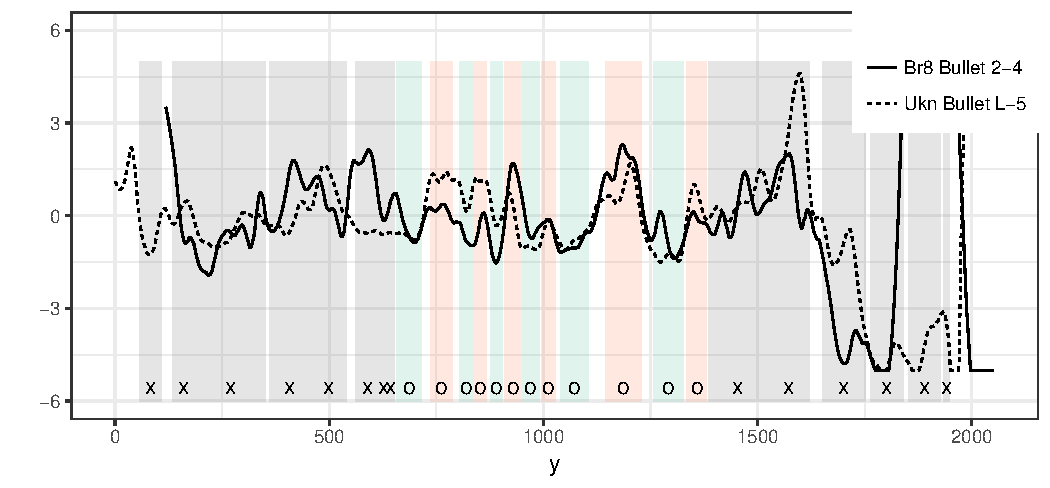
\includegraphics[width=.65\textwidth]{strange-res-1} 

\end{knitrout}
\caption{\label{fig:mismatch}Known mismatch with a relatively large number of maximal consecutive matching striae (twelve) in the middle. The pattern in the middle does look surprisingly similar, however the outer ends of the signatures easily reveals this comparison as mismatch. }
\end{figure}

For smaller numbers of CMS, the percentage of false positives quickly increases. However, if we take other features of the image into account, we can increase the number of correct matches considerably: Figure~\ref{fig:densities} gives an overview of the densities of all of the features derived earlier, distinguishing between known matches (KM) and known non-matches (KNM). The densities of almost all of the features show strong differences between matches and non matches. For example, a high amount of cross-correlation between two signatures is indicative of a match --  in the Hamby study, only known matches have a cross-correlation of 0.75 or higher. There are 97 land-to-land comparisons with a cross-correlation that high.

\begin{figure}[hbtp]
  \centering
\begin{knitrout}
\definecolor{shadecolor}{rgb}{0.969, 0.969, 0.969}\color{fgcolor}
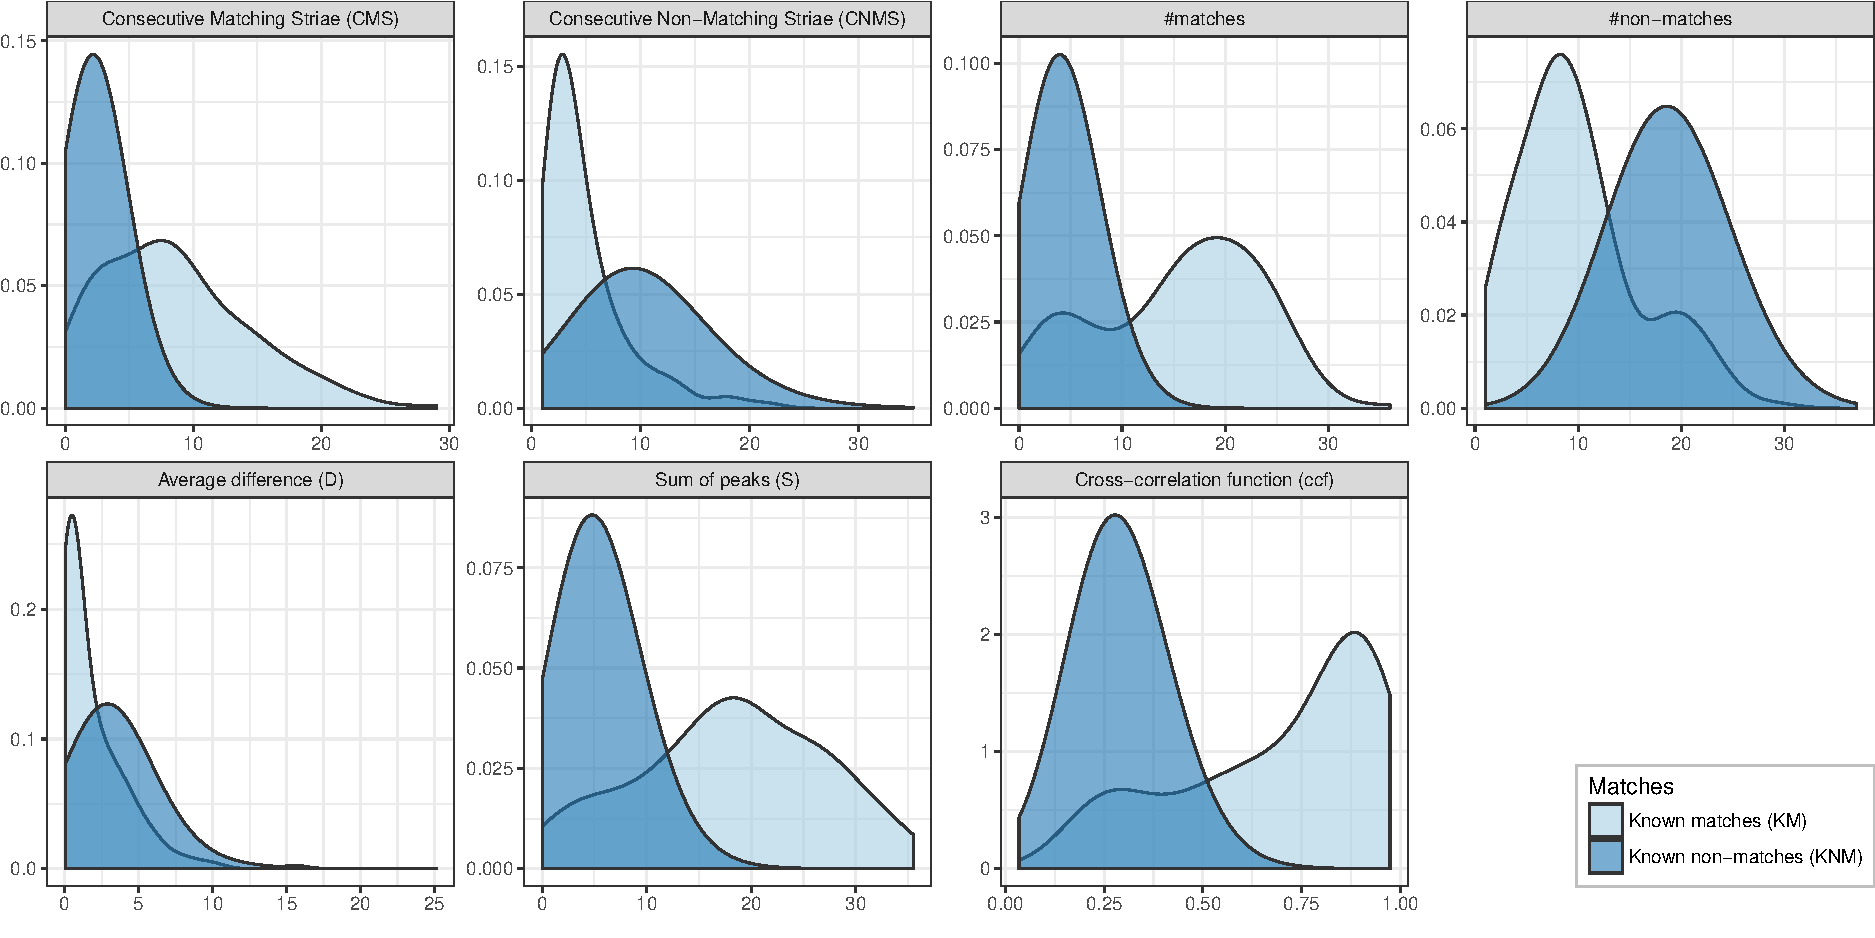
\includegraphics[width=\textwidth]{density-overview-1} 

\end{knitrout}
\caption{\label{fig:densities}Overview of all the marginal densities for features described in section~\ref{sec:algorithm}. Shifts in the mode of the density functions between known matches and known non-matches indicate the variable's predictive power in distinguishing matches and non-matches. Predictive power is shown in more detail in Figure~\ref{fig:rocs}.}
\end{figure}

%' \begin{figure}[hbtp]
%'   \centering
%' <<ratios-overview,echo=FALSE, warning=FALSE, fig.width=12, fig.height=6, out.width='\\textwidth'>>=
%' library(reshape2)
%' dens.stats <- dm %>% group_by(var, variable) %>% mutate(
%'   sum = sum(value, na.rm=TRUE),
%'   up = cumsum(value)/sum,
%'   down = 1 - cumsum(value)/sum
%' )
%' levels(dens.stats$variable) <- c("KM", "KNM")
%' ratios <- dens.stats %>% group_by(var, x) %>% summarise(
%'   lower = sum(up[variable=="KM"], na.rm=TRUE)/sum(up[variable=="KNM"], na.rm=TRUE),
%'   upper = sum(down[variable=="KM"], na.rm=TRUE)/sum(down[variable=="KNM"], na.rm=TRUE)
%' )
%' rm <- melt(ratios, measure.var=c("lower", "upper"))
%' rm$value <- pmin(pmax(rm$value, 0.1), 10)
%' levels(rm$variable) <- c("P(X < c | KM) / P(X < c | KNM)", "P(X > c | KM) / P(X > c | KNM)")
%' qplot(x, value, colour=variable,  data=rm, geom="line", group=variable, 
%'       size=I(1)) + xlab("X") +
%'   facet_wrap(~var, scales="free", ncol=4) + 
%'   scale_y_log10(limits=c(1/10,10)) + theme_bw() + 
%'   geom_hline(yintercept=1, size=0.5) + 
%'   scale_colour_brewer("Estimated Ratios", palette="Set2") + 
%'   ylab("(Logged) Probability Ratios") +
%'   theme(legend.position=c(1,0), legend.justification = c("right", "bottom"),
%'         legend.background = element_rect(colour="grey75"),
%'         plot.margin = unit(c(0,0,0,0), unit="cm")) 
%' @
%' \caption{\label{fig:ratios}Estimated probability ratios for all of the features described in section~\ref{sec:algorithm}. Ratios are logged and and artificially constrained to an interval between (1/10 and 10). Large deviations from one, indicate a strong distinction between matches and known matches based on the variable. Both left tail and right tail probabilities are shown. }
%' \end{figure}

\begin{figure}[hbtp]
  \centering
\begin{knitrout}
\definecolor{shadecolor}{rgb}{0.969, 0.969, 0.969}\color{fgcolor}
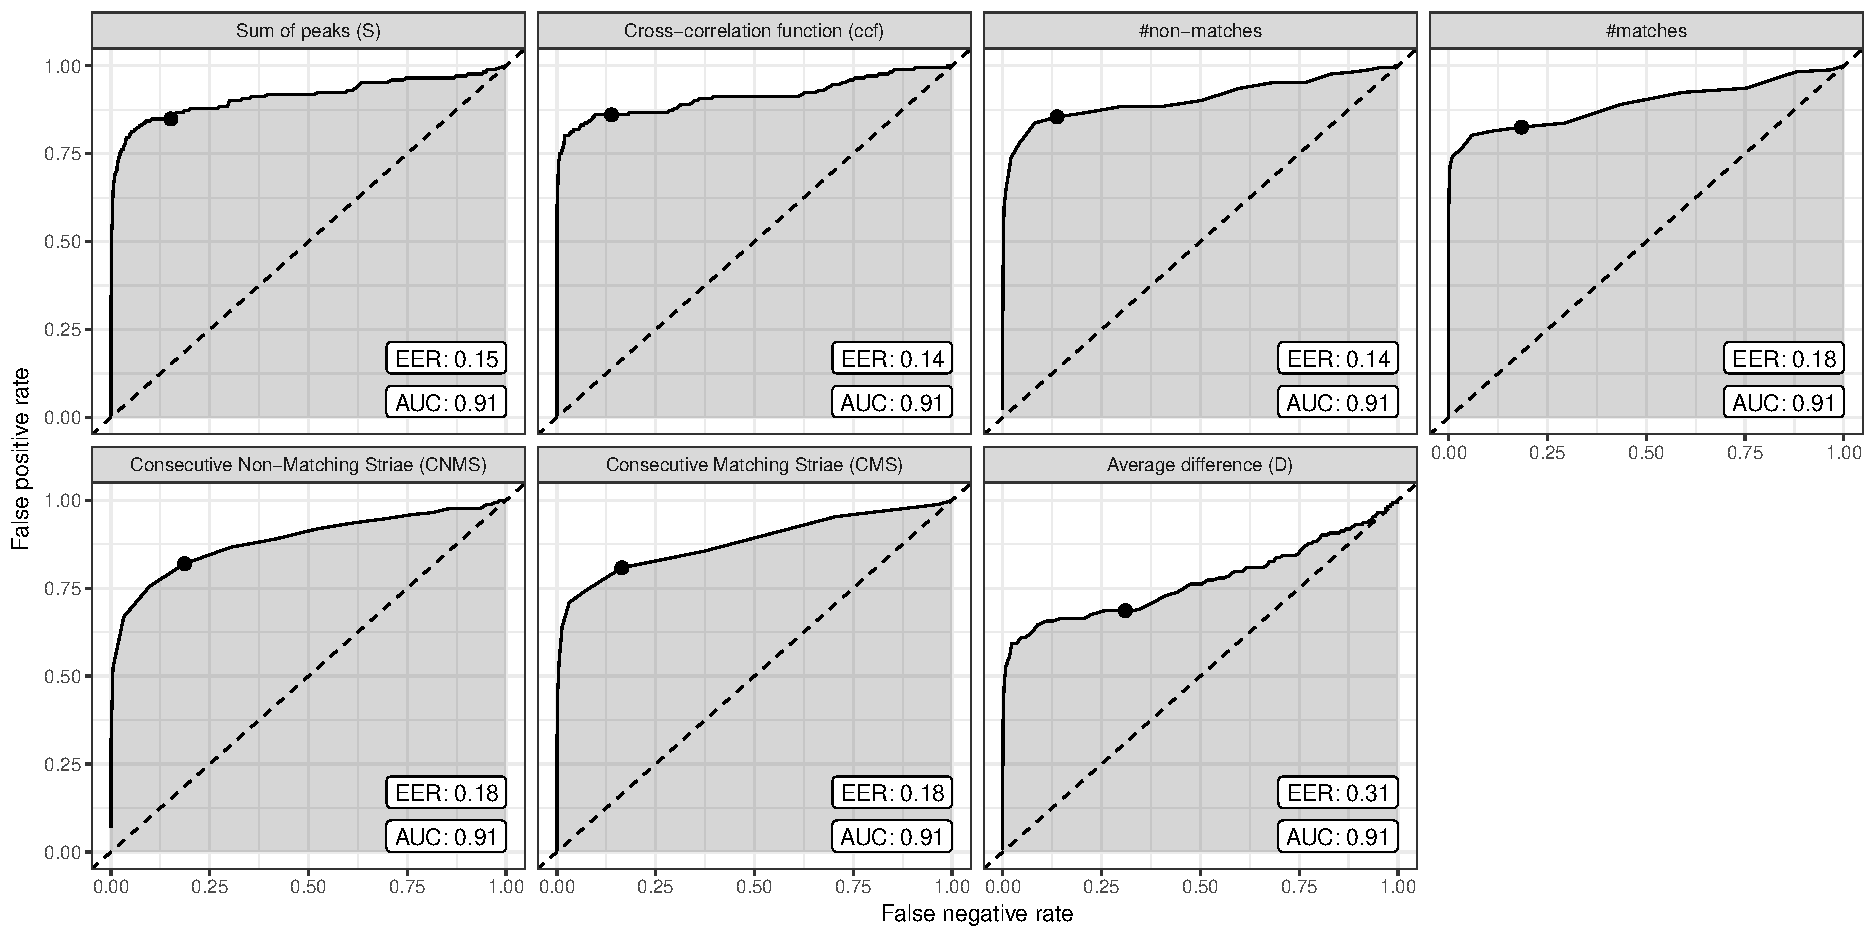
\includegraphics[width=\textwidth]{rocs-overview-1} 

\end{knitrout}
\caption{\label{fig:rocs}ROC curves for all of the features described in section~\ref{sec:algorithm}. Variables are sorted according to their area under the curve (AUC). Except for the distance $D$ between signatures, all individual features derived from the surface measurements and the aligned striation marks are more predictive than the maximal CMS. }
\end{figure}


%' \begin{figure}[hbtp]
%'   \centering
%' \begin{subfigure}[t]{\textwidth}\centering
%' \caption{\label{fig:D}Relationship between maximal CMS and distances between cross sections.}
%' <<D, echo=FALSE, fig.width=8, fig.height=4, out.width='.5\\textwidth'>>=
%' ggplot(data=bstats) + 
%'     geom_jitter(aes(x=factor(CMS), y=D, colour=match), alpha=0.5) +
%'    facet_wrap(~match, labeller="label_both") + xlab("maximum CMS") + 
%'   ylab("Distance between cross sections") +
%'   scale_colour_brewer(palette="Paired") +
%'   theme_bw() + 
%'   theme(legend.position="none") +
%'     xlab("maximum CMS")
%' @
%' \end{subfigure}
%' \begin{subfigure}[t]{\textwidth}\centering
%' \caption{Densities of distances between cross sections for Known Matches (KM) and Known Non Matches (KNM).}
%' <<crosscut-densities, echo=FALSE,  fig.width=7, fig.height=3.5, out.width='.5\\textwidth'>>=
%' ggplot(data=bstats) + 
%'     geom_density(aes(x=D, fill=match), alpha=0.5) +
%'   xlab("Distances between cross sections") +
%'   scale_fill_brewer("", palette="Paired") +
%'   theme_bw() + 
%'   theme(legend.position=c(1,1), legend.justification=c(1,1),
%'         legend.background = element_rect(fill=alpha('white', 0.4))) 
%' 
%' 
%' 
%' x <- seq(0,20, by=0.02)
%' km <- sm.density(bstats$D[bstats$match], display="none", eval.points=x)
%' knm <- sm.density(bstats$D[!bstats$match], display="none", eval.points=x)
%' dframe <- data.frame(x = x, km=km$estimate, knm=knm$estimate)
%' dframe$kmtail <- rev(cumsum(rev(dframe$km)))/sum(dframe$km)
%' dframe$knmtail <- rev(cumsum(rev(dframe$knm)))/sum(dframe$knm)
%' 
%' densities <- data.frame(
%'   match = rep(c("KM", "KNM"), each=(length(x)+2)),
%'   x = rep(c(0, x, 29), times = 2),
%'   estimate = c(0, km$estimate, 0, 0, knm$estimate,0))
%' 
%' ggplot() +
%'   geom_polygon(aes(x=x, y=estimate, fill=match, group=match), colour="black",
%'                data=densities, alpha=0.5) +
%'   xlab("Distances between cross sections") +
%'   scale_fill_brewer("", palette="Paired") +
%'   ylab("Density estimates") +
%'   theme_bw() + 
%'   theme(legend.position=c(1,1), legend.justification=c(1,1),
%'         legend.background = element_rect(fill=alpha('white', 0.4))) +
%'   geom_line(aes(x=x, y=pmin(0.2, kmtail/knmtail/10)), data=dframe) 
%' 
%' @
%' \end{subfigure}
%' \caption{Relationship between distances between cross sections. A small distance between cross sections is indicative of matches between lands.}
%' \end{figure}

%' \begin{figure}[hbtp]
%'   \centering
%' \begin{subfigure}[t]{\textwidth}\centering
%' \caption{\label{fig:ccfs-match}Relationship between maximal CMS and cross-correlation between cross sections.}
%' <<ccfs-match, echo=FALSE, fig.width=8, fig.height=4, out.width='.5\\textwidth'>>=
%' ggplot(data=bstats) + theme_bw() + 
%'   geom_jitter(aes(x=factor(CMS), y=ccf, colour=match), alpha=.5) + 
%'   facet_wrap(~match, labeller="label_both") + 
%'     scale_colour_brewer(palette="Paired") +
%'   xlab("maximum CMS") + ylab("Cross-correlation") +
%'   theme(legend.position="none")
%' @
%' \end{subfigure}
%' \begin{subfigure}[t]{\textwidth}\centering
%' \caption{Densities of distances between cross sections for Known Matches (KM) and Known Non Matches (KNM).}
%' <<ccf-densities, echo=FALSE,  fig.width=7, fig.height=3.5, out.width='.5\\textwidth'>>=
%' ggplot(data=bstats) + 
%'     geom_density(aes(x=ccf, fill=match), alpha=0.5) +
%'   xlab("Cross-correlation between cross sections") +
%'   scale_fill_brewer("", palette="Paired") +
%'   theme_bw() + 
%'   theme(legend.position=c(1,1), legend.justification=c(1,1),
%'         legend.background = element_rect(fill=alpha('white', 0.4))) 
%' @
%' \end{subfigure}
%' \begin{subfigure}[t]{\textwidth}\centering
%' \caption{Ratio of probabilities of $P(ccf > x \mid KM) / P(ccf > x \mid KNM)$.}
%' <<ccf-ratio, echo=FALSE,  fig.width=7, fig.height=3.5, out.width='.5\\textwidth'>>=
%' x <- seq(0,1, by=0.001)
%' library(sm)
%' km <- sm.density(bstats$ccf[bstats$match], display="none", eval.points=x)
%' knm <- sm.density(bstats$ccf[!bstats$match], display="none", eval.points=x)
%' dframe <- data.frame(x = x, km=km$estimate, knm=knm$estimate)
%' dframe$kmtail <- rev(cumsum(rev(dframe$km)))/sum(dframe$km)
%' dframe$knmtail <- rev(cumsum(rev(dframe$knm)))/sum(dframe$knm)
%' 
%' densities <- data.frame(
%'   x = rep(c(0, x, 1), times = 2),
%'   estimate = c(0, km$estimate, 0, 0, knm$estimate,0),
%'   match = rep(c("KM", "KNM"), each=1003))
%' 
%' ggplot() +
%'   geom_polygon(aes(x=x, y=estimate, fill=match), colour="black",
%'                data=densities, alpha=0.5) +
%'   xlab("Cross-correlation between cross sections") +
%'   scale_fill_brewer("", palette="Paired") +
%' #  scale_colour_brewer("", palette="Paired", labels=c("KNM", "KM")) +
%'   theme_bw() + 
%'   ylab("Density estimate") +
%'   theme(legend.position=c(.975,1), legend.justification=c(1,1),
%'         legend.background = element_rect(fill=alpha('white', 0.4))) +
%'   geom_line(aes(x, pmin(5, kmtail/knmtail)), data=dframe) 
%' @
%' \end{subfigure}
%' \caption{A large cross-correlation between cross sections is indicative of matches between lands.}
%' \end{figure}

Similarly, the Euclidean distance $D$ between two signatures is strongly correlated to known matches. Out of the 48 pairs of land-to-land signatures with a distance of less than .25, 47 correspond to known matches (the single known mismatch consists of a pair of signatures that both are very flat with peaks and valleys of less than 1.5$\mu m$). %The average distance between known matches in the Hamby study is $1.86\mu m$ with a standard deviation of $2.31\mu m$; while known mismatches have an average  distance of  $3.27\mu m$ with a standard deviation of $1.93\mu m$.
All of the features in Figure~\ref{fig:densities} show large, if not significant, differences between matches and non-matches. The predictive power of each one of these features is shown in the form of the Receiving Operating Characteristic (ROC) curves in Figure~\ref{fig:rocs}. The features are arranged in descending order according to the area under the curve (AUC). The feature with the highest individual predictive power is $S$, the sum of the average heights of two signatures at peaks and valleys. The maximal number of CMS is only in the seventh position here. The overall high AUC values indicate, that we can successfully employ machine learning methods to distinguish matches from non-matches.
%Table~\ref{tab:importance} shows an overview in the averages and corresponding standard deviations of the set of feature variables derived in section~\ref{sec:algorithm} from the 3D topological surface measurements. There are quite large differences in these averages, indicating 

Using recursive partitioning, we fit a decision tree~\citep{breiman:1984, rpart, rpart.plot} to predict matches between lands based on features derived from the image files. The resulting tree is shown in Figure~\ref{fig:tree}. A total of 132 lands is being matched correctly. Interestingly, the number of consecutive matching striae does not feature in this evaluation. 
Instead of CMS, cross-correlation (ccf) between the signatures is very important in the matching process  by the decision tree. Aside from  cross correlation, the total number of matches is also included in the decision rule. 
Between cross-correlation and CMS, cross-correlation has higher  predictive power. This  does not  contradict earlier findings emphasizing the value of CMS on visual assessments of bullet matches: in those papers, assessments were based on purely visual inspection of either actual bullets or 2D microscopic images of bullets.
Neither one of these methods allows for an assessment of cross-correlations. This is one of the benefits of switching to a digitized version of the images that preserves the 3D surface structure. The findings about the discriminating power of cross-correlation is consistent with the results of the study by \citet{ma:2004}. However, in this study authors did not consider the number of matches and non-matches.

\begin{figure}[hbtp]
  \centering
\begin{knitrout}
\definecolor{shadecolor}{rgb}{0.969, 0.969, 0.969}\color{fgcolor}
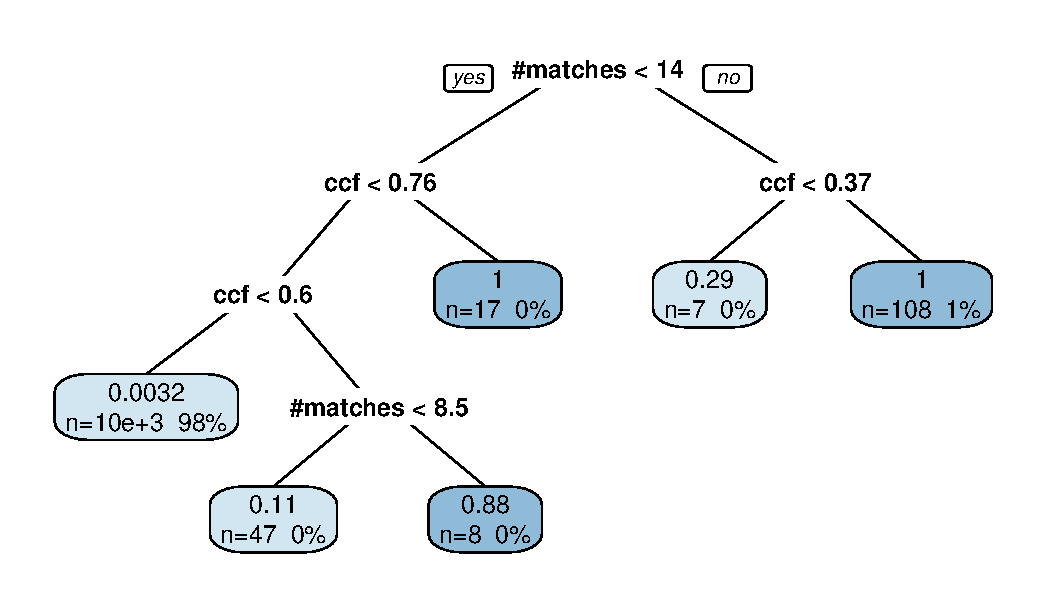
\includegraphics[width=.7\textwidth]{tree-1} 

\end{knitrout}
\caption{\label{fig:tree}Decision tree of matching bullets based on recursive partitioning. The rectangular nodes are the leaves, giving a short summary consisting of the number of observations in the leaf (bottom left), the corresponding percentage of the total (bottom right). The number at the top shows the fraction of these observations that are a match. A 1 or a 0 therefore indicate a homogeneous (or perfect) node. }
\end{figure}




Another benefit of the digitized version of the images is that we can apply several hundred decision trees to combine in a random forest~\citep{breiman:2001, randomForest}.  For each of the trees in a random forest, only two thirds of the observations are used for fitting, while  the remaining third is used to evaluate the tree's predictive power and accuracy, or its reverse, the error rate. Because errors are determined from the one third of held-back observations, this error rate is called the out-of bag (OOB) error. 
Figure~\ref{fig:oob} shows the cumulative out-of-bag error (OOB) rate for 300 trees. 
%
\begin{figure}[hbtp]
  \centering
\begin{knitrout}
\definecolor{shadecolor}{rgb}{0.969, 0.969, 0.969}\color{fgcolor}
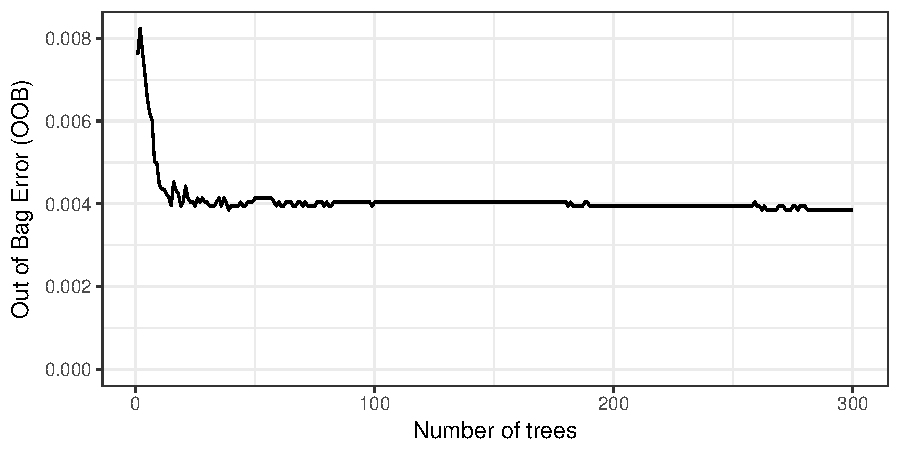
\includegraphics[width=.7\textwidth]{oob-1} 

\end{knitrout}
\caption{\label{fig:oob}Cumulative out-of-bag error rate of a random forest fit to predict land-to-land matches from image features.}
\end{figure}
%
After about 100 trees, the error rate of land-to-land comparisons stabilizes at 0.0039. This is a weighted average between false positive error rate of 0.0001 and an error rate of false negatives of 0.2267. This out-of-bag error rate is over-estimating the actual error in the Hamby study: here, the final random forest based on 300 trees is able to correctly predict all known  matches and non-matches (see Figure~\ref{fig:tree-forest}).
Note that this error rate is based on land-to-land comparisons and is much lower for bullet-to-bullet matches. In the case of the Hamby study, even for the single tree the overall error rate is zero, if we require for a bullet match that at least two of a bullet's lands are matched. % (see Figure~\ref{fig:treeresult}). 
%' \begin{figure}[hbtp]
%'   \centering
%' <<overall-tree, echo=FALSE, fig.width=7, fig.height=4, out.width='.5\\textwidth'>>=
%' bstats$bullet <- gsub("-[0-9]$", "", bstats$b2)
%' bullets <- bstats %>% filter(match, !flagged) %>% group_by(bullet) %>% summarize(
%'   n = n(),
%'   pred = sum(pred > 0.5),
%'   forest = sum(forest > 0.5)
%' )
%' library(reshape2)
%' bm <- melt(data=bullets, id.var=c("bullet", "n"))
%' 
%' bm$prediction <- c("Tree", "Random Forest")[as.numeric(bm$variable)]
%' qplot(data=bm, 100*value/n, reorder(bullet, value/n), size=I(2.5), 
%'       shape=prediction, colour=prediction, alpha=I(0.6)) + 
%'   theme_bw()  + ylab("") + 
%' #  scale_shape_manual(values=c(1,2)) +
%'   scale_x_continuous("Percent of correctly predicted land-to-land matches", 
%'                      breaks = c(0,25,50,75,100), limits=c(0,100)) +
%'   theme(legend.position = "bottom")
%' @
%' \caption{\label{fig:treeresult}Overall predictions for each bullet based on the decision tree (maximum possible number is 12, except for Q and B, where the maximum is 11). Both results for the tree and the random forest are shown. In the tree, at least \hh{40\% of all possible} lands of a bullet are  matched correctly, while the random forest achieves perfect results. Unknown bullet B is the hardest for the tree to match.}
%' \end{figure}
%' %
This makes the errors in the automated approach smaller than the human error in the Hamby study. Out of the 507 participants, who returned results, eight (out of $15 \times 507 = 7,605$) bullets were not matched conclusively, corresponding to a rate of 0.0011. 
%\hh{XXX calling this a false negative rate is problematic. FEs will be up in arms, because inconclusive doesn't necessarily mean something was missed, it could also mean that there was something wrong with the bullets. XXX }

However, error rates based on bullet-to-bullet matches do not carry a lot of weight because of the small size of the study: fifteen unknown bullets are successfully matched to two pairs of ten bullets. Matching bullets can only be tested realistically in a much bigger experiment. 
Another thing to note about  the random forest's error rates is that they are based on probability cutoffs of 0.5, i.e.\ whenever the predicted probability of a match exceeds 0.5, a match is declared. Basing this decision on 0.5 is not necessary. In practice, examiners are allowed a third option of `inconclusive'. On a probability spectrum of outcomes we could therefore introduce an interval of `inconclusive' results in the middle of the spectrum -- which turns out to be not necessary in the Hamby study, because, here, the results from the random forest are very clear cut. Figure~\ref{fig:tree-forest} shows a comparison of the predicted probabilities of a match by the tree and the random forest. %\hh{The tree predicts 132 known matches correctly, with 40 false negatives and one false positive match. The random forest predicts all 172 known matches correctly as well as all 10,212 known non-matches.} 
%Overall, there is a lot of agreement; out of 10,800 land-to-land comparisons, only four cases result in a different decision. 

\begin{figure}[hbtp]
  \centering
\begin{knitrout}
\definecolor{shadecolor}{rgb}{0.969, 0.969, 0.969}\color{fgcolor}
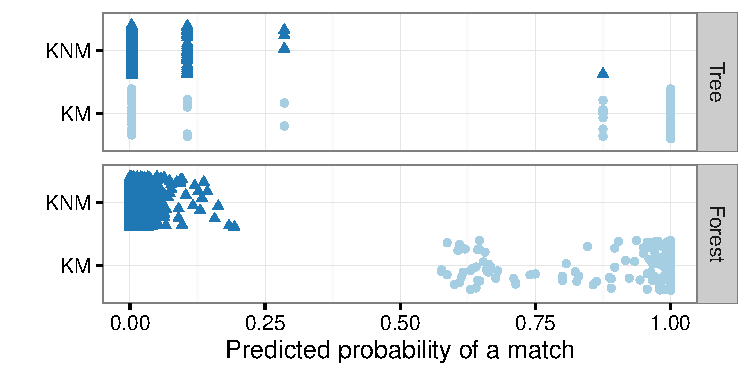
\includegraphics[width=.6\textwidth]{treeforest-1} 

\end{knitrout}
\caption{\label{fig:tree-forest}Prediction results from the tree and the forest. Using a cut-off probability of 0.5 the forest correctly predicts every single comparison. Compared to the tree, the forest's prediction probabilities are  shrunk towards either end of the prediction range. }
\end{figure}

Besides resulting in a probabilistic quantification of matches, random forests also provide an assessment of the importance of each of the features derived from the bullets' 3D topological surface measurements. Figure~\ref{fig:importance} shows an overview of the importance of each variable measured as the mean decrease in the Gini index when the variable in question is included in a tree (for the exact values please refer to Supplement section~\ref{supp:randomforest}). 
\begin{figure}
\begin{knitrout}
\definecolor{shadecolor}{rgb}{0.969, 0.969, 0.969}\color{fgcolor}
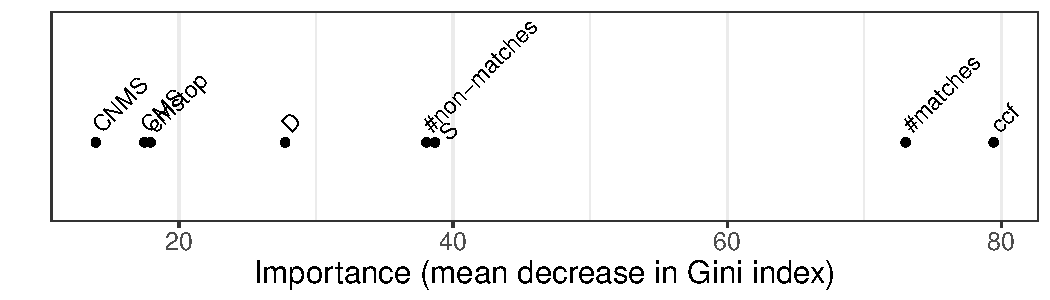
\includegraphics[width=.7\textwidth]{unnamed-chunk-1-1} 

\end{knitrout}
\caption{\label{fig:importance}Importance of features in the random forest. Importance is measured in terms of mean decrease in gini index when including the variable in a decision tree.}
\end{figure}


%The rows in the table are ordered according to descending importance. 
The variables with the most predictive power are cross-correlation and the overall number of matches, followed by the total depth of joint striations $S$ and total number of non-matches. CMS is found only in sixth place.

Besides including results from known matches against known non-matches, we can increase the number of comparisons in the Hamby study to include all possible land-to-land comparisons. This effectively doubles the number of data points available. Comparisons not previously included in fitting the random forest can also be used as an additional source for assessing error rates.  Results for this and a more detailed discussion can be found in Supplement section~\ref{supp:extended}.

\section{Conclusion}

We have presented an algorithm which detects the most prominent but least relevant structure of a bullet from a ballistics identification perspective, removes these features, and produces residuals which allow for the easy identification of markings. We have generalized this algorithm to align the residuals from two bullets to automatically determine whether they are matches. We created a random forest model using many of the features to provide a probabilistic assessment of the quality of a match, along with the most relevant features. %Finally, we have provided an easy-to-use open-source backend, and web frontend to many of these features.

The matching algorithm is sensitive to the parameter choices made. The heights at which signatures are extracted (currently 25$\mu m$ apart) to evaluate stability, as well as the cross-correlation factor (currently 0.95) we set as a minimum threshold do affect the final outcome. Another parameter that must be selected is the amount of smoothing when identifying peaks and grooves (currently, a window of 23.4375$\mu m$ is used, corresponding to a window of 7 values to the left and the right of an observation). While we tried to lay out in the paper the impact that each of the parameter choices has on the matching performance, we are still far from an optimized scenario. 

The Hamby study serves as our evaluation `database'. It consists of only  35 bullets -- this is obviously not a particularly realistic scenario for an automatic matching procedure, but for now we are unaware of other databases containing bullets in the x3p format.
 
The feasibility of creating a database of ballistic images that could be used to identify guns used in crimes was evaluated in a 2008 report~\citep{nap:2008} by the National Research Council. The evaluation was investigating the scalability of NIBIN (National Integrated Ballistic Information Network), which uses proprietary matching algorithms provided by IBIS. The bottomline of the report was that in spite of the many technical and practical hurdles, solutions to all but one problem could be found. The problem that remained is that statistically, the quality of the matching algorithm (in this case, of breech-face marks and firing pin impressions) could not withstand a hugely increased number of records while still maintaining a reasonable workload for forensic examiners, who have to examine possible matches suggested by the system. 
The findings of the NRC report on ballistic imaging are based on two-dimensional greyscale images, which the committee argued were not reliable enough for distinguishing between fine marks. This finding coincides with the assessment by \citet{dekinder:2004} based on the IBIS Heritage system. A further re-assessment by \citet{deceuster:2015} came to the same conclusions based on the EvoFinder system. 
The NRC report also found, that results from 2D images can be improved when matches are based on 3D images. This is consistent with the importance of features found here: out of the top five features (see Figure~\ref{fig:importance}), only the total number of matches and mismatches are available for a match based on 2D features.

By suggesting an automated algorithm that first removes class characteristics, such as the grooves and the curvature of the bullet to reveal the region of the  land, then identifies peaks and valleys on this land, we reduce subjectivity and with it possible sources of bias. In particular, `the concept of counting striations is subjective and based on experience'~\citep{miller:1998}.

For a fair assessment of the performance of an algorithm, we need transparency. Our matching  algorithm is open: the code is readily available in form of the R package x3prplus~\citep{x3prplus}, and the code to produce this paper is available at \url{http://www.github.com/erichare/imaging-paper}. To understand whether an automated approach along the lines of the one we propose can accurately identify sets of bullets with undistinguishable markings, it will be necessary to assemble a much larger database that includes a wide range of ammunition types, degrees of damage, gun makes, etc. We are unaware of the existence of any such database. In addition to serving as a realistic testbed for the performance of the automated matching algorithm, such a database would also permit testing the underlying, as of yet untested, assumptions of uniqueness and reproducibility of the markings left by a gun on bullets.

%\hh{XXX speed? XXX}

An approach that might be helpful comes from Biometrics \citep{jain:2015:tphil, jain:2015}. It has been successfully applied in the Aadhar project (the effort by the Unique Identification Authority of India (UIDAI) to provide a unique 12-digit identification number to approximately 1.2 billion residents of India based on ten fingerprints and two irises).
This approach uses dictionary learning based on small square patches  of 64x64 or 32x32 pixels. For matching bullets, a simpler, one-dimensional window approach might be sufficient to match striation marks because of the physical forces  leading to the existence of these marks.  

\section*{Acknowledgment} 
Thanks to David Baldwin for pointing us to the NIST database and doing a Ballistics 101 for us.
Thanks to the men and women behind the software R~\citep{R}, and the authors of the R packages  knitr~\citep{knitr} and ggplot2~\citep{ggplot2}.



% AOS,AOAS: If there are supplements please fill:
%\begin{supplement}[id=suppA]
%  \sname{Supplement A}
%  \stitle{Title}
%  \slink[doi]{10.1214/00-AOASXXXXSUPP}
%  \sdatatype{.pdf}" 
%  \sdescription{Some text}
%\end{supplement}

\bibliographystyle{imsart-nameyear.bst}
%\biboptions{authoryear}
\bibliography{references}


\end{document}
